%%%%%%%%%%%%%%%%%%%%%%%%%%%%%%%%%%%%%%%%%%%%%%%%%%%%%%%%%%%%%%%%%%%%%
%% This is a (brief) model paper using the achemso class
%% The document class accepts keyval options, which should include
%% the target journal and optionally the manuscript type.
%%%%%%%%%%%%%%%%%%%%%%%%%%%%%%%%%%%%%%%%%%%%%%%%%%%%%%%%%%%%%%%%%%%%%
\documentclass[journal=jpcbfk,manuscript=article]{achemso}

%\documentclass[english,aps,preprint,pre,floatfix,nofootinbib,showpacs,showkeys]{revtex4-1}
%%%%%%%%%%%%%%%%%%%%%%%%%%%%%%%%%%%%%%%%%%%%%%%%%%%%%%%%%%%%%%%%%%%%%
%% Place any additional packages needed here.  Only include packages
%% which are essential, to avoid problems later. Do NOT use any
%% packages which require e-TeX (for example etoolbox): the e-TeX
%% extensions are not currently available on the ACS conversion
%% servers.
%%%%%%%%%%%%%%%%%%%%%%%%%%%%%%%%%%%%%%%%%%%%%%%%%%%%%%%%%%%%%%%%%%%%%
\usepackage[version=3]{mhchem} % Formula subscripts using \ce{}

\SectionNumbersOn

%include hyperlinks to figures
\documentclass{article}
\usepackage{graphicx}
\usepackage[%  
    colorlinks=false,
    pdfborder={0 0 0},
    linkcolor=blue
]{hyperref}

\usepackage{amsmath}
\usepackage{amssymb}
\usepackage{color}
\usepackage{CJK}
\usepackage{framed}
\usepackage[hidelinks]{hyperref}
\usepackage{algorithm}
\usepackage{algpseudocode}
\algdef{SE}[DOWHILE]{Do}{doWhile}{\algorithmicdo}[1]{\algorithmicwhile\ #1}

\usepackage[scaled=0.85]{beramono}
\usepackage[T1]{fontenc}
\usepackage{changepage}
\usepackage{mathrsfs}

%%%%%%%%%%%%%%%%%%%%%%%%%%%%%%%%%%%%%%%%%%%%%%%%%%%%%%%%%%%%%%%%%%%%%
%% If issues arise when submitting your manuscript, you may want to
%% un-comment the next line.  This provides information on the
%% version of every file you have used.
%%%%%%%%%%%%%%%%%%%%%%%%%%%%%%%%%%%%%%%%%%%%%%%%%%%%%%%%%%%%%%%%%%%%%
%%\listfiles

%%%%%%%%%%%%%%%%%%%%%%%%%%%%%%%%%%%%%%%%%%%%%%%%%%%%%%%%%%%%%%%%%%%%%
%% Place any additional macros here.  Please use \newcommand* where
%% possible, and avoid layout-changing macros (which are not used
%% when typesetting).
%%%%%%%%%%%%%%%%%%%%%%%%%%%%%%%%%%%%%%%%%%%%%%%%%%%%%%%%%%%%%%%%%%%%%

\makeatletter
    \setlength\@fptop{0\p@}
\makeatother

\newcommand*\mycommand[1]{\texttt{\emph{#1}}}

\newcommand{\state}[1]{$\mathcal{S}_{#1}$}


\newcommand*{\rood}[1]{#1}
\newcommand*{\blauw}[1]{#1}
\newcommand*{\groen}[1]{#1}
\newcommand*{\blauwr}[1]{#1}
\newcommand{\Expect}[1]{\mathrm{E}\left[#1\right]}
\newcommand{\norm}[1]{\left\lVert#1\right\rVert}

%\newcommand*{\addref}[1]{\textcolor{red}{\{ADD REF: #1\}}}

\newcommand*{\noter}[1]{\textcolor{red}{[[#1]]}}		% notes on
%\newcommand*{\noter}[1]{}					% notes off

%\usepackage[draft]{todonotes}   % notes shown
\usepackage[disable]{todonotes} % notes hidden
\usepackage{comment}

\usepackage[normalem]{ulem}
\usepackage{algorithm}
\usepackage{subfig}
\usepackage{algpseudocode}

%%%%%%%%%%%%%%%%%%%%%%%%%%%%%%%%%%%%%%%%%%%%%%%%%%%%%%%%%%%%%%%%%%%%%
%% Meta-data block
%% ---------------
%% Each author should be given as a separate \author command.
%%
%% Corresponding authors should have an e-mail given after the author
%% name as an \email command. Phone and fax numbers can be given
%% using \phone and \fax, respectively; this information is optional.
%%
%% The affiliation of authors is given after the authors; each
%% \affiliation command applies to all preceding authors not already
%% assigned an affiliation.
%%
%% The affiliation takes an option argument for the short name.  This
%% will typically be something like "University of Somewhere".
%%
%% The \altaffiliation macro should be used for new address, etc.
%% On the other hand, \alsoaffiliation is used on a per author basis
%% when authors are associated with multiple institutions.
%%%%%%%%%%%%%%%%%%%%%%%%%%%%%%%%%%%%%%%%%%%%%%%%%%%%%%%%%%%%%%%%%%%%%
\author{Michael S. Jones}
\affiliation{%
  Pritzker School of Molecular Engineering, %
  The University of Chicago, %
  929 East 57th Street, Chicago, Illinois 60637, United States%
}

\author{Brennan Ashwood}
\affiliation{%
  Department of Chemistry, Institute for Biophysical Dynamics, and James Franck Institute, %
  The University of Chicago, %
  929 East 57th Street, Chicago, Illinois 60637, United States%
}

\author{Andrei Tokmakoff}
\affiliation{%
  Department of Chemistry, Institute for Biophysical Dynamics, and James Franck Institute, %
  The University of Chicago, %
  929 East 57th Street, Chicago, Illinois 60637, United States%
}

\author{Andrew L. Ferguson}
\email{andrewferguson@uchicago.edu}
\affiliation{%
  Pritzker School of Molecular Engineering, %
  The University of Chicago, %
  929 East 57th Street, Chicago, Illinois 60637, United States%
}

%\author{I. Ken Groupleader}
%\altaffiliation{A shared footnote}
%\email{i.k.groupleader@unknown.uu}
%\phone{+123 (0)123 4445556}
%\fax{+123 (0)123 4445557}
%\affiliation[Unknown University]
%{Department of Chemistry, Unknown University, Unknown Town}
%\alsoaffiliation[Second University]
%{Department of Chemistry, Second University, Nearby Town}

%\author{Susanne K. Laborator}
%\email{s.k.laborator@bigpharma.co}
%\affiliation[BigPharma]
%{Lead Discovery, BigPharma, Big Town, USA}

%\author{Kay T. Finally}
%\affiliation[Unknown University]
%{Department of Chemistry, Unknown University, Unknown Town}
%\alsoaffiliation[Second University]
%{Department of Chemistry, Second University, Nearby Town}

%%%%%%%%%%%%%%%%%%%%%%%%%%%%%%%%%%%%%%%%%%%%%%%%%%%%%%%%%%%%%%%%%%%%%
%% The document title should be given as usual. Some journals require
%% a running title from the author: this should be supplied as an
%% optional argument to \title.
%%%%%%%%%%%%%%%%%%%%%%%%%%%%%%%%%%%%%%%%%%%%%%%%%%%%%%%%%%%%%%%%%%%%%
\title[]{Applying State-free Reversible VAMPNets and Markov State Models to Learn Dynamics of DNA Oligonucleotides}


%%%%%%%%%%%%%%%%%%%%%%%%%%%%%%%%%%%%%%%%%%%%%%%%%%%%%%%%%%%%%%%%%%%%%
%% Some journals require a list of abbreviations or keywords to be
%% supplied. These should be set up here, and will be printed after
%% the title and author information, if needed.
%%%%%%%%%%%%%%%%%%%%%%%%%%%%%%%%%%%%%%%%%%%%%%%%%%%%%%%%%%%%%%%%%%%%%
%\abbreviations{IR -- infrared, NMR -- nuclear magnetic resonance, UV -- ultraviolet}
%\keywords{Takens}

\begin{document}
%%%%%%%%%%%%%%%%%%%%%%%%%%%%%%%%%%%%%%%%%%%%%%%%%%%%%%%%%%%%%%%%%%%%%
%% The manuscript does not need to include \maketitle, which is
%% executed automatically.  The document should begin with an
%% abstract, if appropriate.  If one is given and should not be, the
%% contents will be gobbled.
%%%%%%%%%%%%%%%%%%%%%%%%%%%%%%%%%%%%%%%%%%%%%%%%%%%%%%%%%%%%%%%%%%%%%

\newpage

\begin{abstract}

Despite rapid advances in DNA nanotechnology and a robust understanding of the associated thermodynamics, the sequence-dependent mechanisms of DNA hybridization are not fully understood. In this work, we investigate these dynamics by performing equilibrium coarse-grained simulations of oligonucleotide sequences with varied G:C placement. We employ State-Free Reversible VAMPnets to directly learn the slowest dynamical modes of each sequence and optimize Markov State Models (MSMs) construction. Furthermore, we perform elevated temperature simulations to recapitulate temperature-jump IR and FTIR data collected on the oligonucleotides. For repetitive sequences, we find a spectrum of slow dynamics associated with out-of-register base pairing and kinetically relevant transitions between these states. In contrast, G:C pairs near the center of the duplex induce more rapid fraying dynamics. In both cases, hybridization/dissociation mechanisms deviate from an “all-or-nothing” model. Our computational predictions are in excellent accord with experiment, and provide new fundamental understanding of the sequence-dependent kinetics and mechanisms of DNA hybridization.

% revise "excellent accord" above?

\noindent \url{https://www.overleaf.com/project/5e9e5110c524b8000192c548}

\end{abstract}
%%%%%%%%%%%%%%%%%%%%%%%%%%%%%%%%%%%%%%%%%%%%%%%%%%%%%%%%%%%%%%%%%%%%%
%% Start the main part of the manuscript here.
%%%%%%%%%%%%%%%%%%%%%%%%%%%%%%%%%%%%%%%%%%%%%%%%%%%%%%%%%%%%%%%%%%%%%

\newpage

\section{\label{sec:intro}Introduction}

Over the last couple decades, DNA has proved to be much more than a vessel for genetic information. From sensing, to computing, to directed self-assembly, the programmable and predictable nature of DNA has unlocked numerous unforeseen nanotechnology applications \citep{Seeman2017DNANanotechnology, Adleman1994MolecularProblems, Rothemund2006FoldingPatterns, Gu2010ALine}. DNA dynamical behavior has become increasingly important in these technologies and a point of focus in fundamental biological processes such as transcription and gene regulation.  \citep{Deluca2020DynamicDevices, Cordes2010SensingTransfer, Naimark2020DNADevelopment}. Our understanding of DNA hybridization -- the formation of a duplex from two amenable single strands -- has been integral to these developments. The effect of sequence on hybridization thermodynamics has been rigorously explored, and nearest-neighbor calculations can account for many mismatched pairs, dangling ends, and other non-native bonding effects \citep{SantaLucia1998AThermodynamics, Santalucia2004TM}. Secondary DNA structures such as hairpins and G-quadruplexes have also been studied in depth and leveraged for nanotechnology applications \citep{Tsukanov2013DetailedOrigami, Mosayebi2014TheFormation, Mergny2019DNANanotechnology}. Although many experimental and computational studies have investigated DNA dynamical phenomena from the picosecond to millisecond range, the sequence-dependent mechanisms of hybridization and dissociation dynamics are not fully understood \citep{Yin2011KineticsHybridization, Xiao2019, Hinckley2014Coarse-grainedEffects, Sanstead2016, Porschke1971CooperativeTransition, Porschke1973ThermodynamicsPairs, Chen2007InfluenceHybridization, Craig1971ElaxationOligon}. Moreover, it is unclear the extent to which these processes evolve in an "all-or-nothing" fashion or if an ensemble metastable states facilitates the transition \citep{Araque2016LatticeCooperativity, Sikora2013ModelingIntermediates}.

Our understanding of hybridization dynamics has been built from decades of experiments -- such as temperature-jump, salt-jump, pH-jump, or other perturbative methods -- that drive DNA out of equilibrium and monitor relaxation processes in one direction \citep{Morrison1993SensitiveSolution, Wetmur1968KineticsDNA, Craig1971ElaxationOligon, Porschke1973ThermodynamicsPairs, Williams1989LaserDGCATGC, Narayanan2012ExploringMixing, Chen2007InfluenceHybridization, Sanstead2018DirectDehybridization}. More recently, single molecule diffusion and tethered multifluorophore assays have facilitated equilibrium analysis, however these results can be hampered by slow data collection rates and fluorescent tags altering strand dynamics, particularly for shorter oligomers \citep{Liu20173DSolution,  Schickinger2018TetheredHelices, Chen2008Base-by-baseSpectroscopy, Dupuis2013Single-moleculeHelices, Morrison1993SensitiveSolution}. Given that dynamic insights from these experiments are limited, several coarse-grained molecular dynamics (MD) models have been employed to gain further detail \citep{Romano2013DNADependence, Hinckley2013AnHybridization, Maciejczyk2014DNAModel, Markegard2015}. Although these models provide experimentally verified speed-ups compared to all-atom simulations, the long timescales on which DNA hybridization and dissociation events occur can still make these processes difficult to sample via direct simulation techniques \citep{Phys2014}. Instead, many previous studies of DNA hybridization have employed accelerated sampling methods such as metadynamics, umbrella sampling,  transition path sampling, and forward flux sampling \citep{Schmitt2013ExploringSurface, Sambriski2009,  Hoefert2011MolecularOligonucleotides, Romano2013DNADependence}. Simplified lattice models can expedite computation time and yield useful thermodynamics and transition state information, however some configurations may not be accessible and kinetics are less informative \citep{Araque2016LatticeCooperativity, Phys2019}. Other computational works use dramatically elevated temperature or denaturing solvent concentrations to induce one-way dissociation events \citep{Wong2008TheSimulations, Perez2010Real-timeUnfolding}. Taken together, most experimental and computational work have studied certain aspects the overall dynamics process in one direction or in a biased fashion.

Recent studies have coupled experimental techniques with machine learning (ML) and  MD simulations to investigate and predict sequence-dependent kinetics \citep{Schickinger2018TetheredHelices, Zhang2018PredictingSequence}. Where these studies focus on association and dissociation kinetics alone, we seek to broaden our analysis into higher order dynamical processes and metastable intermediates. For example, metastable out-of-register or "shifted" base pairing in repetitive sequences have been documented in previous computational studies \citep{Phys2014, , Maciejczyk2014DNAModel, Araque2016LatticeCooperativity, Xiao2019}). The extent to which these states are kinetically relevant is difficult to determine experimentally, and appears highly sequences dependent. Frayed structures and dynamics have also been investigated in numerous computational and experimental studies \citep{Zgarbova2014BaseRNA, Nonin1995TerminalFraying, Nikolova2012ProbingSimulations, Andreatta2006UltrafastHelix}. Sanstead et al. highlighted the role of these dynamics during duplex dissociation, where the stability and relaxation timescale of frayed states was dictated by G:C base placement 10-mer oligonucleotide sequences \citep{Sanstead2016}. Together, these dynamics represent the most substantial deviations from all-or-nothing behavior that can be variably expressed via subtle sequence differences in short oligomers.

In this work, we study the same four sequences explored by Sanstead et al in an effort to uncover the sequence-dependent dynamics and their relation to metastable structures mentioned above \citep{Sanstead2016}. We use the coarse-grained 3 Sites per Nucleotide (3spn2) model to simulate hybridization and dissociation behavior near each sequence's melting temperature \citep{Hinckley2013AnHybridization}. We perform these analyses without biasing simulations or assuming that one processes is a strictly reversible version of the another. Furthermore, we leverage the properties of Markov State Models (MSMs) -- namely that conditional probability depends only on the current state of the system \citep{Pande2010EverythingAsk} -- to combine many independent and unbiased trajectories and develop an understanding of sequence-specific kinetics and thermodynamics. MSMs have recently been implemented to study mechanisms and microstate distributions of DNA hybridization  \citep{Jin2019, Xiao2019}, but the slowest sequence-dependent kinetics were not the focus of these studies. \citet{Pinamonti2017} used MSMs to compare the slowest dynamics of short RNA nucleotides and found that stacking timescales are highly sequence dependent \citep{Pinamonti2017}. We take a similar approach to study 10-mer DNA oligonucleotides and introduce State Free Reversible Vampnets (SRVs) to directly learn the slowest sequence-dependent dynamical modes \citep{Chen}. Furthermore, we integrate SRVs into the MSM pipeline by generating an optimized low dimensional basis in which microstate clustering can be performed. We show that SRV coordinates can be useful for both directly interpreting dynamical trends and for improving overall SRV-MSM quality when compared to more conventional methods such as time-structure independent components analysis (tICA).

We find that G:C base pair placement in decamer oligonucleotides has a substantial effect on dynamical behavior. By evaluating equilibrium trajectories we can study the relevance of metastable states during both the hybridization and dissociation process. Because SRVs generate an optimized low dimensional basis, we show that we can access higher resolution MSMs (about a 50\%reduction in required lag time) and generate more detailed models. Additionally, we can compare slow dynamical modes and metastable states between sequence-specific SRV-MSMs. Within these metastable dynamical states, we leverage diffusion maps to analyze the diversity of structures whose inter-conversion rate are too fast to produce unique slow modes. Finally, we run higher temperatures simulations to investigate the temperature-dependent nature of some experimentally relevant dynamical responses. Taken together, our analysis reflects similar results to previous computational and experimental DNA work, while elucidating new insights into sequence-dependent dynamics, metastable structures, and relative timescales. 

%%%%%%%% Intro comments %%%%%%%%%%%%%%%%%

%Progress in DNA science and engineering has been bolstered by a well-established understanding of sequence-dependent thermodynamics. Thousands of DNA and DNA-complex crystal structures have been captured, and the equilibrium structure of every tetranucleotide motif were simulated in a distributed computational effort \citep{Manuscript2014The2012}. Hybridization thermodynamics can predicted with high fidelity by nearest-neighbor stacking, and these calculations have been experimentally verified to account for mismatched pairs, dangling ends, and other non-native motifs \citep{SantaLucia1998AThermodynamics, Santalucia2004TM}.

% Secondary DNA structures such as hairpins and quadruplexes have also been studied in depth and leverage for nanotechnology applications.

%Furthermore several computational models have been paramaterized to capture these thermodynamic characteristics.

%These studies have fueled increasingly complex structural DNA technologies, but developments in dynamic DNA nanotechnologies have outpaced our understanding of the dynamics themselves \citep{Deluca2020DynamicDevices}. Certain dynamical models for hybridization -- such the nucleation-zipper mechanism and fraying-peeling mechanism for dissociation -- have been well-established for decades (\citep{Wetmur1968KineticsDNA, Porschke1971CooperativeTransition}). Although many experimental and computational studies have rigorously explored DNA dynamical phenomena such as hybridization, hairpin formation, and single base pair flipping, the sequence-dependent mechanisms of hybridization and dissociation dynamics are not fully understood \citep{Yin2011KineticsHybridization, Xiao2019, Hinckley2014Coarse-grainedEffects, Sanstead2016, Porschke1971CooperativeTransition, Porschke1973ThermodynamicsPairs, Chen2007InfluenceHybridization, Craig1971ElaxationOligon}. Moreover, it is unclear the extent to which these processes evolve in an "all-or-nothing" fashion or if an ensemble metastable states facilitates the transition \citep{Araque2016LatticeCooperativity, Sikora2013ModelingIntermediates}. 

%Still, rich dynamics have been observed short nucleotides \citep{Sanstead2018DirectDehybridization} and the sequence-dependent effects on these dynamics are not well understood.

%Progress has also been made in modeling kinetics for certain dynamic DNA systems, such as toehold exchanges and optical barcodes \citep{Zhang2009ControlExchange, Shah2019ProgrammingFingerprinting}. Sequence effects on association and dissociation rates were predicted using combined experimental and machine learning approaches, however higher order dynamics are less well understood \citep{Zhang2018PredictingSequence}.  Hairpin \citep{Woodside2006DirectAcid} and in duplex hybridization \citep{yer2014KineticsAT-tracts, Sanstead2016, Sanstead2018DirectDehybridization} studies have revealed sequence-dependent effects and varied differential deviations from "all or nothing" behavior. In temperature-jump spectroscopy, G:C placement alters the slow kinetic response attributed to dissociation and a fast response likely corresponding to terminal A:T fraying. Experimentally, however, it is difficult to pick up on dynamics that have similar spectroscopic signatures and to tease apart temporally close responses that might be combined into one stretched exponential signal. 


% include Tokmakoff conclusions in the intro -- sequence-dependent deviations from two-state behavior. The slow response was attributed to complete strand dissociation, while the fast response described base fraying. We perform longer equilibrium sampling near Tm to get a sense of sequence equilibrium behavior, as well shorter simulations at a range of higher temperatures to replicate T-jump data. Taken together, our analysis reflects similar results to previous computational and experimental DNA work, while elucidating new insights into sequence-dependent dynamics, metastable structures, and relative timescales. 

\section{\label{sec:methods}Methods}

\subsection{\label{sec:methods}Simulation set up}

The 3 site per nucleotide (3spn2) coarse grained model was designed to accelerate DNA computation relative to all-atom models while maintaining experimental melting temperatures, stacking energies, and persistence lengths\citep{Hinckley2013AnHybridization}. Interactions sites are located at phosphate, sugar, and base centers of mass; anisotropic potentials are designed to model non-bonded interactions such as intra-strand base-stacking, inter-strand cross-stacking, and base pairing. The model has been validated against experimentally determined structural properties and hybridization rates, although no dynamic information was used to parameterize the model other than Langevin friction coefficients \citep{Hinckley2013AnHybridization, Hinckley2014Coarse-grainedEffects}. 3spn2 has widely-adopted to study numerous phenomenon including DNA packing in viral capsids, protein-DNA binding, and nucleosome unwrapping. \citep{Cordoba2017AIons, Lu2020OpenAWSEMSummary, Lequieu2016Tension-dependentUnwrapping}. 

We initialized four sequences previously the subject of ultra-fast T-jump experimentation -- 5'ATATATATAT3' (AT-all), 5'GATATATATC3' (GC-end), 5'ATATGCATAT3' (GC-core), and 5'ATGATATCAT3' (GC-mix) -- along with their complementary strands in a periodic box of dimensions 7.774 nm \citep{Sanstead2016, Phys2014}. We specified a 240 mM implicit salt concentration and used a A Debye-Huckel approximation for electrostatic interactions within a 5 nm cutoff. We ran our simulations in the NVT ensemble and fixed temperature via a Langevin thermostat in order to model implicit solvent interactions \citep{Schneider1978Molecular-dynamicsTransitions}. Simulations were conducted at empirically determined  melting temperatures in order to maximize transitions between dissociated and hybridized states. We use a 20 fs time step and $13\times10^{9}$ steps in each simulation, saving frames every 100 ps. For each sequences, 40 simulations were performed in parallel, consuming about 24 serial CPU-hours on 28xIntel E5-2680v4 processors for each simulations. Half of runs were initialized from the hybridized state and half from a dissociated state. The first 10000 frames (1 $\mu$s of simulation time) of each simulation were removed, resulting in 40 x 250000 frames and a total of 1 ms simulation time per sequence. Depending on sequence, we observed between 40-100 hybridizing and dissociating transitions across all runs.

\subsection{\label{sec:methods}Featurization}

All intermolecular pairwise distances for both oligonucleotides were calculated at each frame using the MDtraj software package \citep{McGibbon2015MDTraj:Trajectories}. Intermolecular distances removed translational and rotational symmetries, but additional symmetries arise from the self-complementary nature of these sequences -- both the sense and anti-sense strands are identical to each other. To account for this, we averaged permutable distances (45 pairs in total) together. This permutation reduction follows a similar procedure used in tICAgg coordinates construction \citep{Sengupta2019AutomatedSelf-assembly}. The VAMP-2 scoring method was employed to evaluate the kinetic variance of the feature set and optimize hyperparameters \citep{WuVariationalData, Mardt2018VAMPnetsKinetics}. The VAMP-2 score uses the covariances of a set of inputs estimates the transfer operator of a dynamical system, providing a robust and object means to evaluate various parameters and models.

\begin{figure}[ht!]
	\begin{center}
        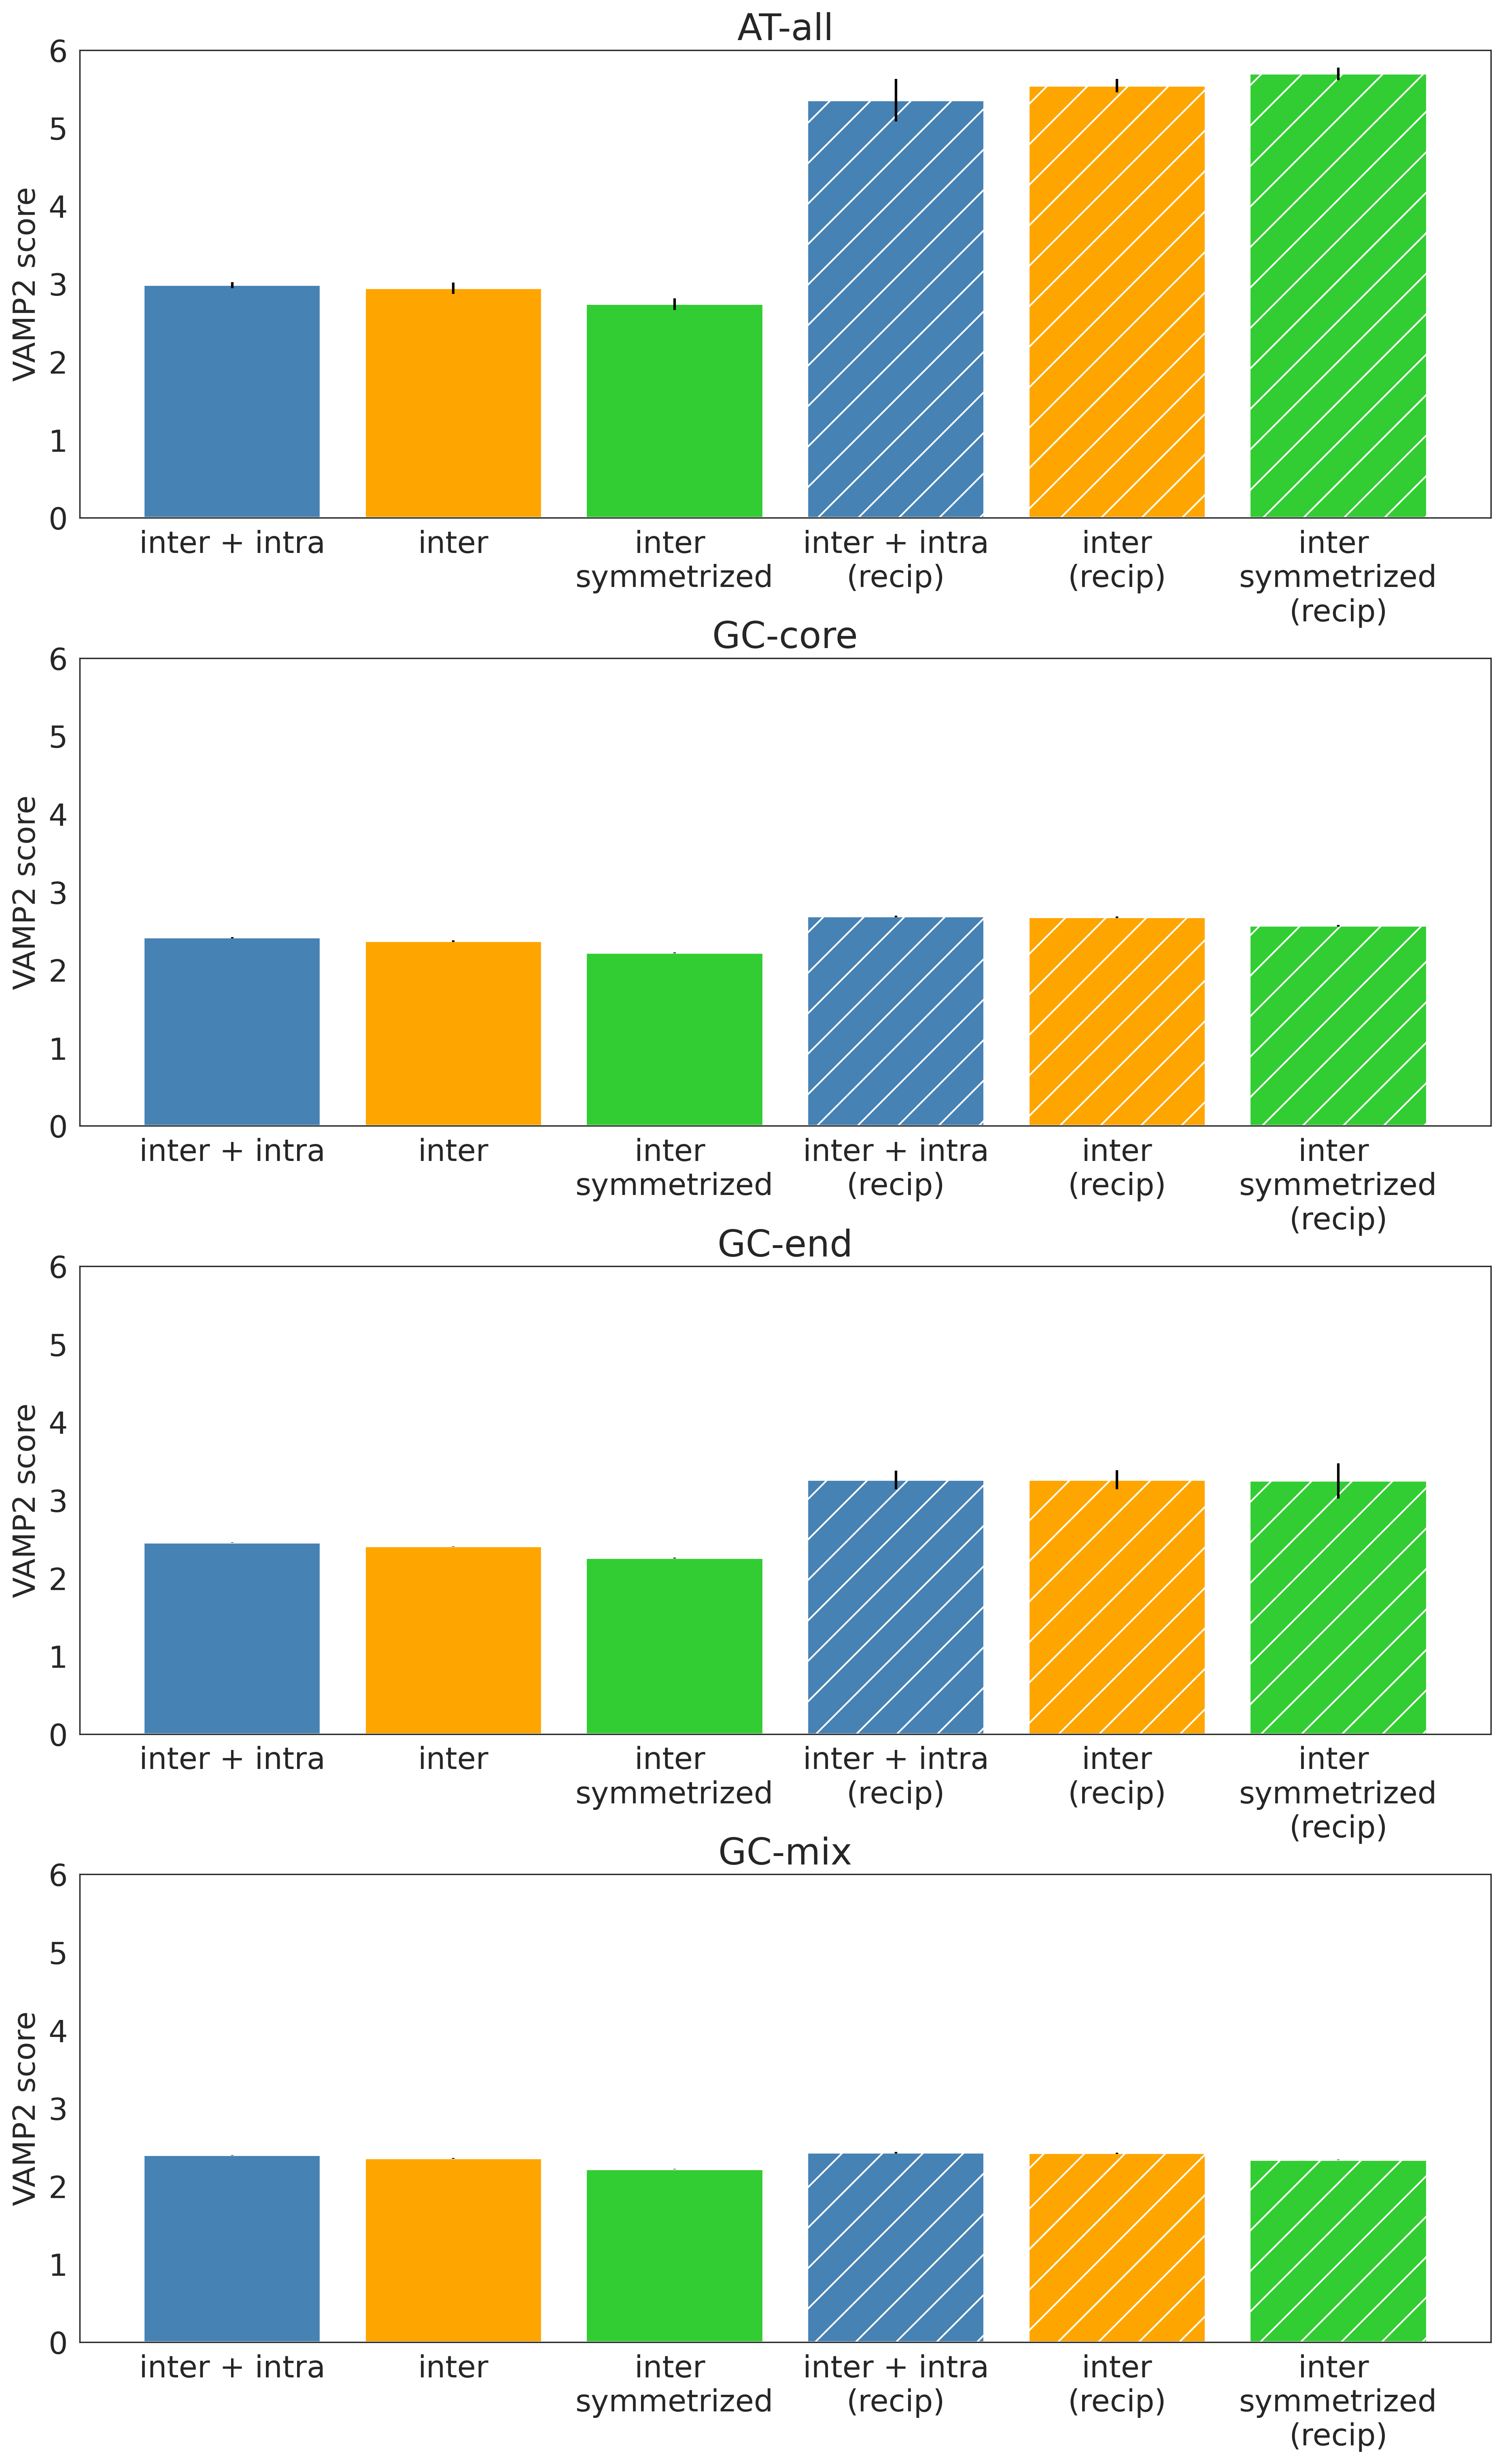
\includegraphics[width=80mm,
        scale=0.5]{Figs/figs_imp/all_permute_vamps_nolegend.png}
        \caption{5-fold cross validation to calculate the VAMP-2 score for each feature set. The inverse distances showed improvement across sequences, and the 55-dimension symmetrized coordinate set performed about as well as larger features set.}
        \label{fig:allseq_features_vamp2}
	\end{center}
\end{figure}

We compared scores for the intermolecular, intra+intermolecular,  and symmetrized intermolecular distances and found small differences between the three that varied by sequences, but overall we did not observe a loss in kinetic information when using the symmetrized feature set (\ref{fig:allseq_features_vamp2}). We found a substantial increase in VAMP-2 score when using reciprocal pairwise distances and chose reciprocal symmetrized coordinates to train the model. The smaller feature set enabled faster training times and better statistics over permutable distances, without appearing to suffer a loss in generality or model resolution. These features were normalized and passed into sequence-specific SRVs. 

\subsection{\label{sec:methods}SRVs}
 
SRVs were first developed by Chen et al. as a means to directly learn slow eigenfunctions of the transfer operator \citep{Chen}. The method is a descendant of VAMPnets \citep{Mardt2018VAMPnetsKinetics}, deep canonical correlation analysis \citep{Andrew2013DeepAnalysis},and extended dynamic mode decomposition with dictionary learning (EDMD-DL) \citep{Li2017ExtendedOperator}. The framework uses a twin-lobed artificial neural network to learn an optimal basis set for the variational approach to conformational dynamics (VAC) from which the leading eigenfunctions of the transfer operator are then estimated \citep{Noe2013ASystems}. The resulting orthogonal modes are associated with the slowest dynamical processes in a system, and can be used to interpret kinetic information directly (such as physical correlations and timescales) and to construct MSMs \citep{Sidky, Pande2010EverythingAsk}. SRVs provide robust nonlinear approximation and computation time that scales linearly with the amount of input data and are more powerful and efficient that tICA and ktICA approaches. This is a key attribute to our system as 10 million frames with 55 features in each frame are used for each sequence. The SRV framework has been tested on toy systems where the true eigenfunctions of the transfer operator are known and on small protein simulation data such as the WW-domain and Trp-cage mini-protein \citep{Chen, Sidky}. For these latter system, SRV-MSMs were contructed in order to find the stability of metastables states as well as transition probabilities between those states.

Using optimized hyperparameters and featurized trajectory data, we transformed 55 reciprocal pairwise distances into a low dimensional SRV basis set. In order to maintain consistency between sequences, we kept all SRV training hyperparameters the same with the exception of the number of outputed slow modes. We determined the number of slow modes via cross-validation on the VAMP-2 score to ensure that the coordinate did not over fit on statistical noise \citep{McGibbon2015VariationalKinetics}. In particular, we looked for convergence in the VAMP-2 score and inconsistency between cross validation scores -- suggesting that the model may be over-fitting on artifacts in the training data. We used a batch size of 50000 and ran each model for a total of 20 training epochs. We used two hidden layers and set the size of each layer to 100. For cross-validation and comparison between different hyper-parameters, we used a 80/20 validation split training. SRV training required about 22 GPU-minutes across 1 GPU and 10 CPUs. SRV training was implemented using Keras and Tensorflow \citep{KerasGithub.Com, Abadi2016TensorFlow:Systems}.

% might want to include these training params in the SI?

\subsection{\label{sec:methods}SRV-MSMs}

MSMs are a powerful tool for interpreting large amounts of simulation data in a statistically robust and experimentally comparable way \citep{Phys2011MarkovValidation, Husic2018MarkovScience}. The technique relies on the discretitization of kinetically similar conformations into microstates and finds the conditional probability between states within some lag time. The reliance on conditional probabilities allows for many independent simulations (longer than the lag time) to be collectively interpreted. To take full advantage of the MSM frameworks, however, the input basis should be as kinetically meaningful as possible \citep{Pande2010EverythingAsk}. Because SRV eigenfunctions translate simulation features into their slowest kinetic representations, they are optimally suited as an MSM basis. To build our SRV-MSM framework, we employed the PyEmma MSM pipeline and generated independent models for each sequence \citep{Scherer2015PyEMMAModels}. In a similar approach to Sidky et al. we performed k-means microstate clustering, Bayesian MSM construction, and PCCA+ hierarchical macrostate assignments \citep{Sidky}. The number of microstates were determined by VAMP-2 score, and the SRV-MSM lag time was selected based on implied timescales convergence.  The number of PCCA+ macrostates was determined based on the characteristic of each system and will be discussed more in depth in the results. Additional step-by-step details on SRV-MSM construction for each sequence are provided in the supplemental information and on Github (https://github.com/mrjoness/...).

%%%%%%%% Methods comments %%%%%%%%%%%%%%%%%

%We found close agreement with explicit ion simulations performed with 240 mM \ce{NaCl} and 18 mM \ce{MgCl2} (supplemental) but 7x slower simulation speed made adequate sampling more difficult to achieve under these conditions.

%We initialized explicit ions such that 240 mM \ce{NaCl} and 18 mM \ce{MgCl2} were added to the box in addition to 18 Na counter ions to balance the charge from the 9 phosphate groups in each oligonucleotide backbone \citep{Hinckley2015}. We used a periodic box size of 7.774 nm and an effective oligo concentration of 7 mM. We used an Ewald summation to calculate long range Coulombic interaction between DNA and ions using a real space cutoff of 2 nm.

% A Debye-Huckle screening potential was used to monitor account for ion concentration . 

\begin{comment} 
% SI equations
In the equations below, we show how covariances are obtained from some featurization $\chi$ of a time series $x_t$ and its time-lagged pairs $x_{t+\tau}$. The VAMP-2 score can then be found for $\chi$ by applying the VAMP principle with cross-validation.

\begin{align*}
 	\mathscr{C}_{00}=&\Expect{\chi(x_t)\chi(x_t)^\intercal}_t\\
 	\mathscr{C}_{01}=&\Expect{\chi(x_t)\chi(x_{t+\tau})^\intercal}_t\\
 	\mathscr{C}_{11}=&\Expect{\chi(x_{t+\tau})\chi(x_{t+\tau})^\intercal}_{t+\tau}\\
	\\
 	VAMP2[\chi]=&\norm{\mathscr{C}_{00}^{-1/2}\mathscr{C}_{01}\mathscr{C}_{11}^{-1/2}}_F^2 +1
 	%VAMP2^{val}[\chi]=&\norm{\mathscr{(C_{00}^{val})}^{-1/2}\mathscr{C}_{01}^{val}\mathscr({C}_{11}^{val})^{-1/2}}_F^2 + 1
\end{align*}\label{CK1}

\end{comment}

%%%%%%%%%%%%%%%%%%%%%%%%%%%%%%%%%%%%%%%%%%%%%%%%%%%%%%%%%%%%%%%%


\section{\label{sec:Results}Results}

% Include analysis on overall hybridization rates here or at the end?
% Show difference between between full hybridization and partial events (GC-end and AT-all)

\subsection{SRV-MSMs provide better resolution than tICA-MSMs} 

\begin{figure}[ht!]
	\begin{center}
        \includegraphics[width=400, scale=1]{Figs/figs_imp/AT-all_implied_timescales.png}
        \caption{SRV-MSM implied timescales converged faster than tICA-MSM implied across the five leading AT-all modes. Timescales are directly compared at the chose lag time of 1.2 ns}
        \label{fig:AT-all_dynamic}
	\end{center}
\end{figure}

As a preliminary check on SRV-MSM performance, we compared implied timescales with a more conventional tICA-MSM approach. Previous work showed that SRV-MSM implied timescales converged faster than tICA-MSM timescales, enabling a shorter lag time and therefore a higher resolution model \citep{Sidky}. Here we observed the same trend across all sequences, and we highlight these results for AT-all in figure \ref{fig:AT-all_dynamic}, emphasizing that faster convergence was observed across all leading timescales. Similar plots for the other sequences are included in the SI. We also note that the infrequency of transitions relative to the individual trajectory length leads to slower convergence of the leading mode. Because this mode corresponds the overall hybridization and dissociation process, we found that it displayed similar behavior across all sequences and that higher order modes were more informative for lag time selection.

%addition to timescale comparison, we found that tICA-MSMs often produced inconsistent PCCA+ clusterings between runs and tended to be less physically meaningfully

\begin{figure}[ht!]
	\begin{center}
        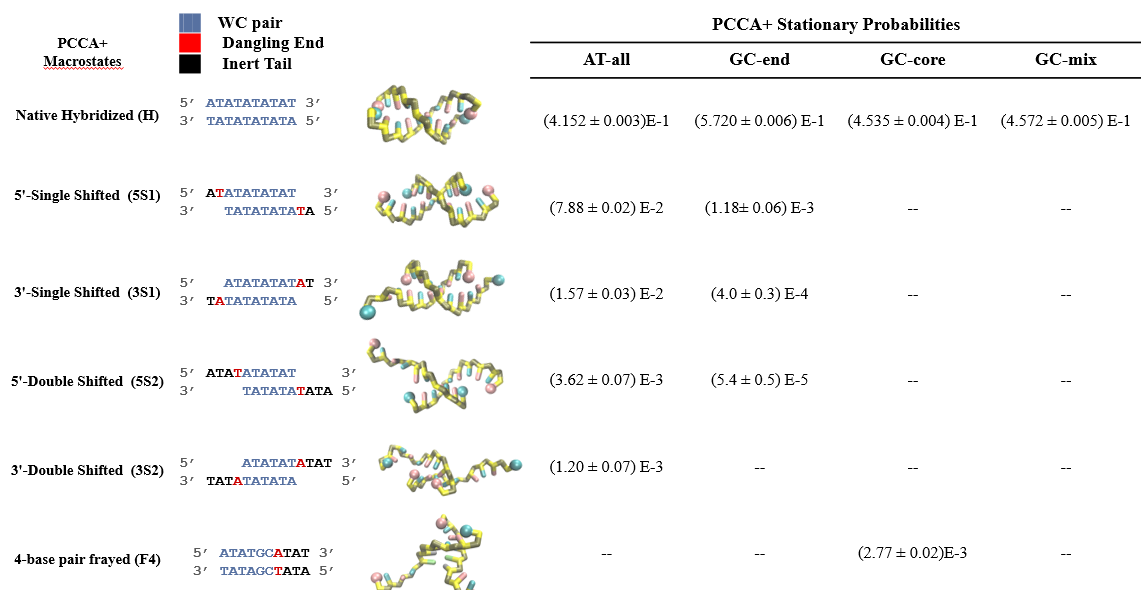
\includegraphics[width=160mm, 
        scale=1]{Figs/figs_imp/allseq_states.png}
        \caption{Nearest neighbor representations, molecular renderings, and sequence-dependent probabilities for PCCA+ macrostates. The dissociated state is not shown but represents the remainder of the stationary probability for each sequence.}
        \label{fig:allseq_table}
	\end{center}
\end{figure}

\begin{figure}[hb!]
	\begin{center}
        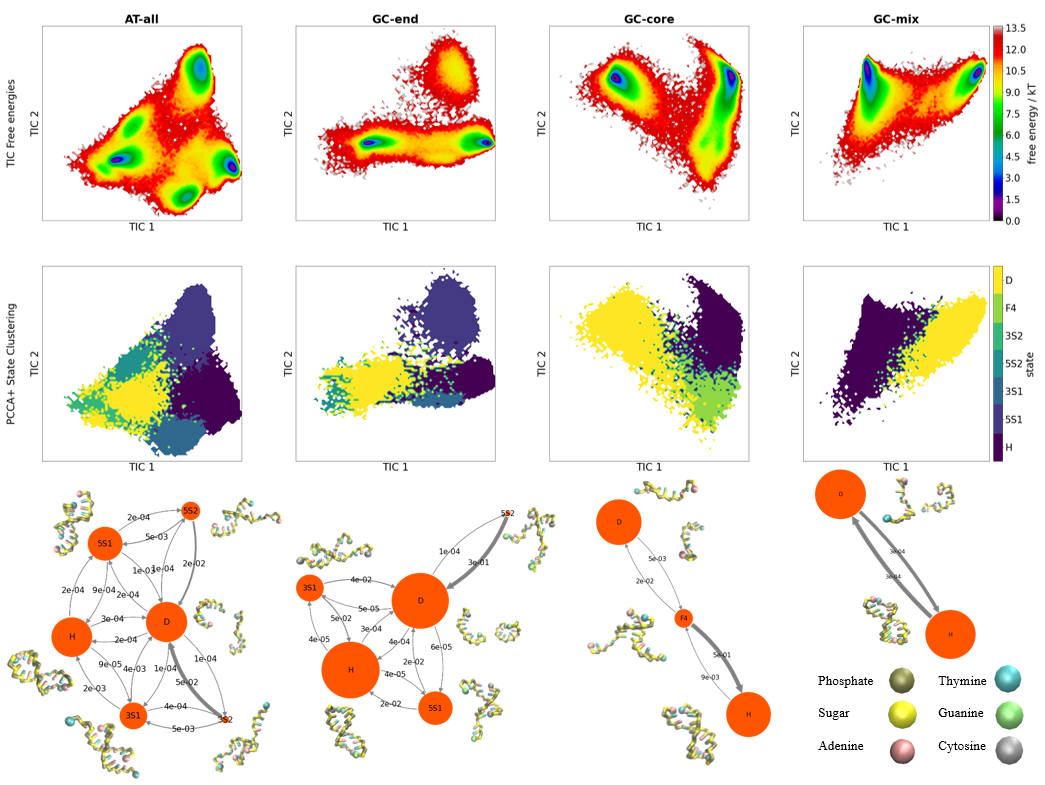
\includegraphics[width=160mm, 
        scale=1]{Figs/figs_imp/allseq_transitions.png}
        \caption{Free energies maps and PCCA+ states clusterings are shown in the tICA space in order to enhance visibility in dimensions. Flux diagram between PCCA+ states are shown for each sequences, accompanied by representative structures are for each state. Arrows indicate the probability of transitioning out of the state within the lag time. Circle areas are proportional to state stability.}
        \label{fig:allseq_transition}
	\end{center}
\end{figure}

\subsection{All SRV-MSMs}

Following the analysis pipeline described above, we generate SRV-MSMs for each sequence. We identified seven kinetically relevant states that are captured within the resolution of the model. These include the fully hybridized state (H) in which all native base pairings are intact, the fully dissociated state (D), four "shifted" states (5S1, 5S2, 3S1, 3S2) where complementary base pairs form out-of-register, and a frayed state (F4), unique to GC-core, in which the four terminal A:T base pairs are unbound. Shifted states are only observed for AT-all and GC-end; state abbreviations indicate the direction of the shifted overhang (5' vs. 3') and the number of shifted motifs relative the native state (1 vs. 2). GC-mix displays two-state behavior within the resolution of the model, however we will show that the hybridization and dissociation are still characterized by an ensemble of shorter-lived states. Stationary probabilities in each of these states are shown in figure \ref{fig:allseq_table}. We also show that PCCA state assignments are capturing free energy minima in tICA space as independent states.

% rewrite this into one paragraph
\subsection{Shifted state stability}

The repetitive AT motifs in the AT-all and GC-end sequences produces a collection of out-of-register states similar to those shown in previous coarse-grained and all-atom studies \citep{Phys2014,  Romano2013DNADependence, Araque2016LatticeCooperativity, Xiao2019}. The thermodynamic stability of these states can be evaluated against experimental prediction by defining each structure in terms of "dangling ends" -- unpaired bases adjacent to the paired duplex -- and "inert tails" -- free bases that extend beyond the dangling end \citep{Michele2014EHybridization}. Dangling ends tend to have small stabilizing effects, and inert tails decrease stability as they increase in length -- 3' inert tails have stronger effects than 5' tails. Although sequence-dependent effects of inert tails are less well known, dangling end effects can be factored into nearest neighbor (NN) calculations \citep{Santalucia2004TM}. It is informative to compare our MSM predictions against NN calculations to understand how inert tail or kinetic effects cause deviation from these predictions. For AT-all, NN calculations (figure \ref{fig:NN_table}) predict that conformations in the 5' shifted states (5S1 and 5S2) are more energetically favorable than those in the 3' shifted state (3S1 and 3S2). We find qualitative agreement to our PCCA+ free energies, where inert tail effects likely contribute a 4-6.5 kJ/mol increase in free energy compared to dangling end predictions alone. For GC-end, we consider C:T and G:A mismatches in the GC-ends shifted states as non-interacting dangling ends such that each shifted conformation has four total dangling ends. Based on this treatment, NN calculations yield higher overall free energies (due to fewer native base pair contacts), but, contrary to PCCA+ results, predict that 3' out-of-register states to be more stable than 5' states. This leads us to believe that 5' vs. 3' differences -- attributed to some combination of 5' tails preferentially stacking on the core duplex and 3' tails perturbing the duplex structure -- may out-weight NN stacking effects alone \citep{Doktycz1990ThermodynamicATGC}. 

% and inert tails tend to decrease stability as they increase in length, particularly at lower ionic strengths. It has been shown that 5' dangling ends with one inert tail have higher melting temperatures and are energetically favorable compared to 3' ends \citep{Senior1988InfluenceDuplexes, Dickman2012ThermodynamicDNAs}. These effects might be attributed to some combination of 5' tails preferentially stacking on the core duplex and 3' tails perturbing the duplex structure \citep{Doktycz1990ThermodynamicATGC}. 

% Although NN calculations predict 5' vs. 3' stabilities for AT-all, we observe that GC-end 5S1 state remains more populated than the 3S1 state contrary to NN predictions. Indeed, we do not observe the formation of a stable 3S2 state for GC-end, further indicating that these states 3' states are unfavorable. This leads us to believe that 5' vs. 3' differences -- attributed to some combination of 5' tails preferentially stacking on the core duplex and 3' tails perturbing the duplex structure -- may out-weight NN effects \citep{Doktycz1990ThermodynamicATGC}. 

\begin{figure}[ht!] % right place for NN table? could go to SI
	\begin{center} 
        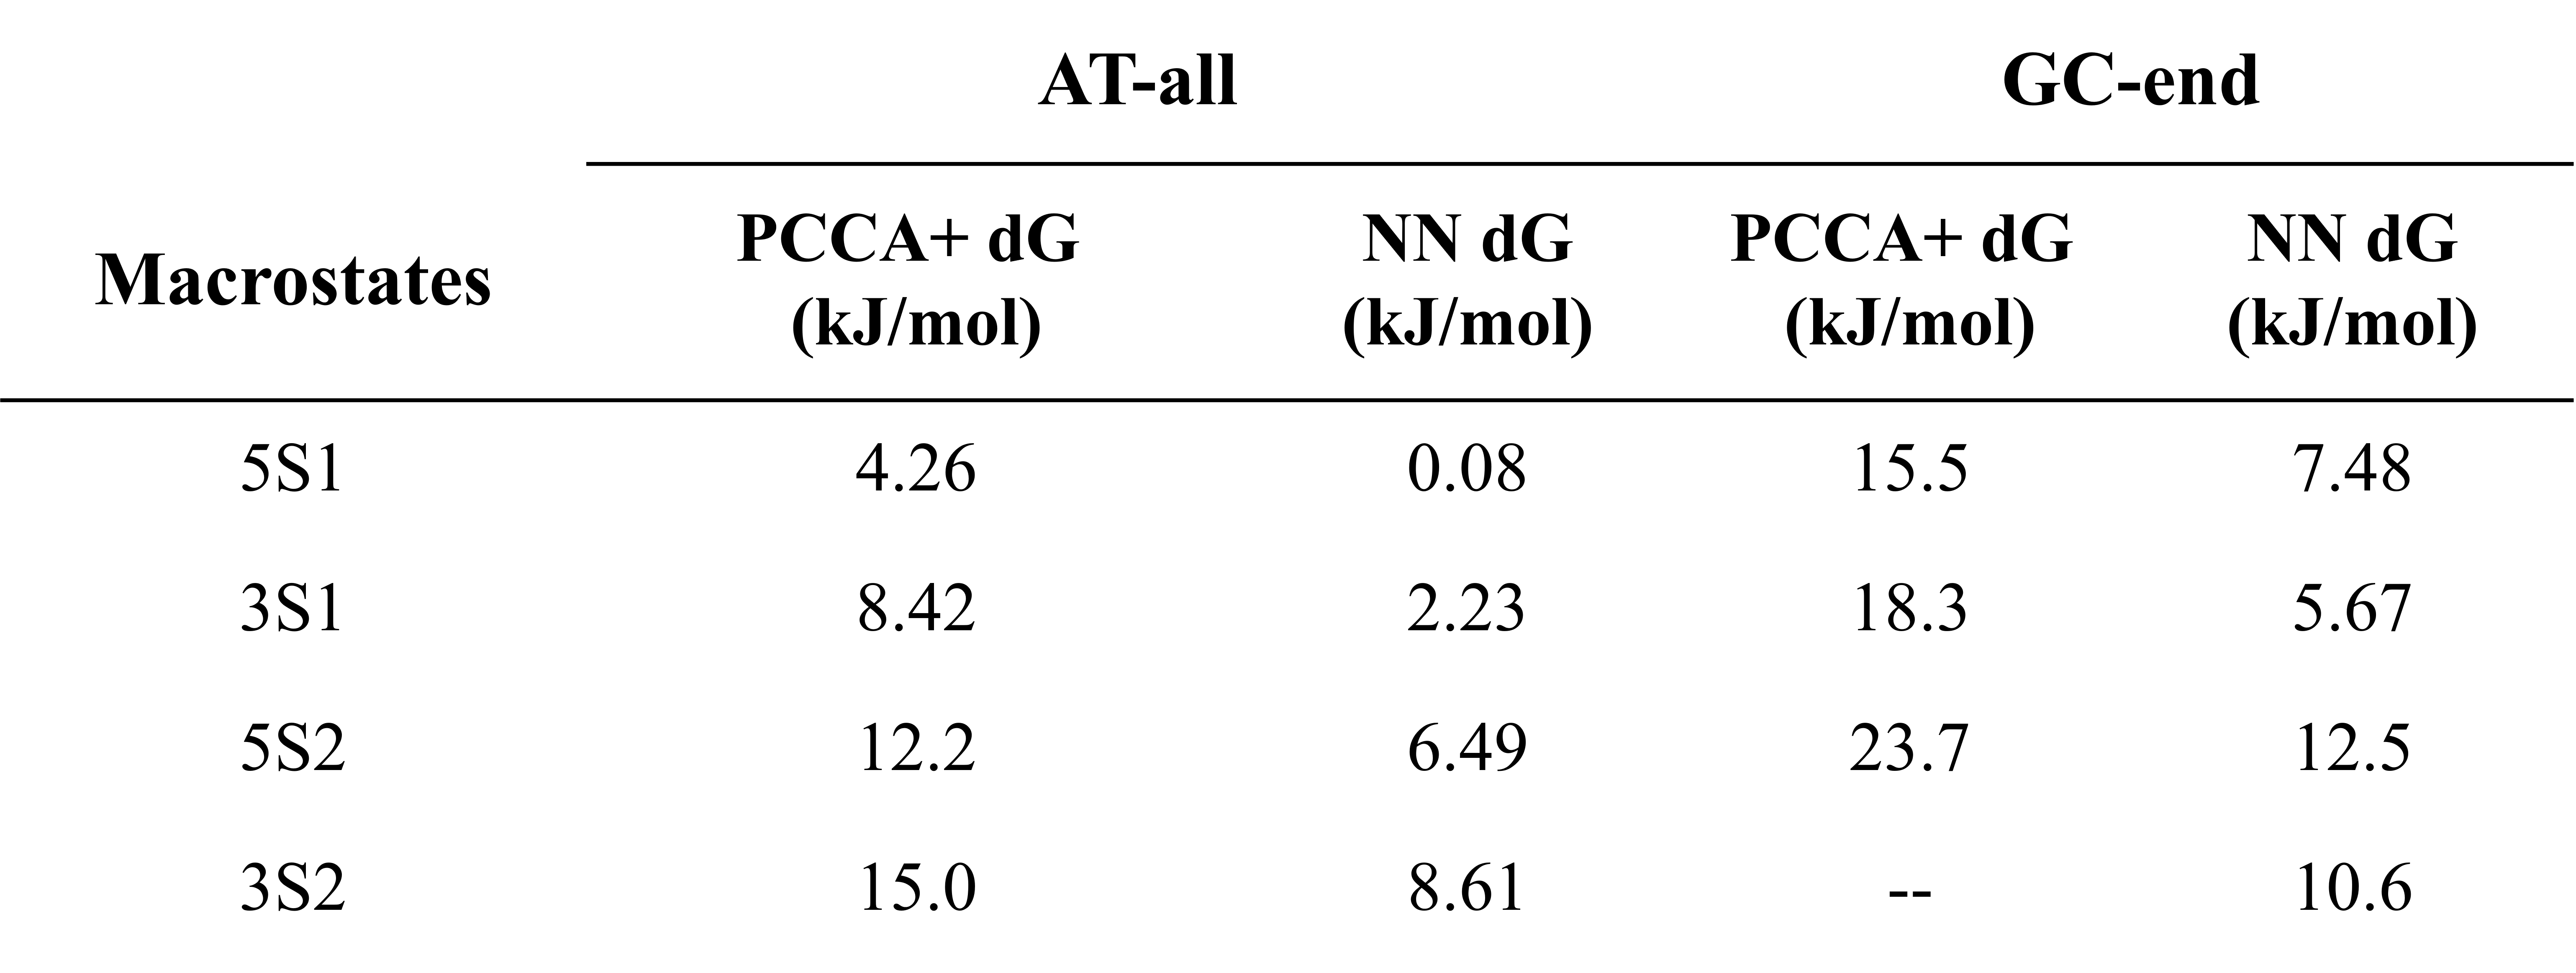
\includegraphics[width=100mm, scale=1]{Figs/figs_imp/shifted_FE_table.png}
        \caption{Comparisons between free energies based on simulation macrostate populations and nearest neighbor calculations. All free energies are normalized such that that the native hybridized state is set to zero. Calculations included dangling end contributions but do not take inert tails effects.}

        \label{fig:NN_table}
	\end{center}
\end{figure}

%if AT-all has highest frequency and GC-end has lowest then can describe role of metastable states as increasing rate for the former but decreasing rate for the later (for kinetic traps that do not terminate in native hybridization and delay the process as a whole).

\subsection{Shifting dynamics}
%\subsubsection{Transition probabilities between states}

Beyond state probabilities and free energy approximations, the coarse-grained MSM yields valuable discrete kinetic information in the form of transition probabilities between states. Figure \ref{fig:allseq_transition}!!!change ref!!! shows the probability of moving from one state to another within the MSM lag time. For AT-all, we observe approximately equal probability of transitioning from D to any other state, indicating that this is primarily a diffusion-driven process. Once a transition has been made, however, the 5' vs. 3' overhang and degree of shifting play an important role in determining whether the duplex will continue to shift out-of-register or re-dissociate. Transition probabilities are higher when moving towards a more aligned state than towards a more shifted state -- 5S1 $\rightarrow$ H is more favorable than 5S1 $\rightarrow$ 5S2, suggesting that these metastable shifted states play a more significant role in facilitating the hybridization process than dissociation. Furthermore, we see equal or higher transition probability from shifted states to the dissociated state (5S1 $\rightarrow$ D) than to more aligned states (5S1 $\rightarrow$ H), indicating that the shifting-hybridization process is frequently disrupted by complete dissociation. In particular, we observe that the transition probability 3S2 $\rightarrow$ D is 10x higher than 3S2 $\rightarrow$ 3S1. Indeed for GC-end, we observe no significant flux between the 5S2 state and the structural similar 5S1 state, indicating that the former acts more as a kinetic trap than a pathway to H. The 5S1 and 3S1 states still readily convert with H, however there is an order of magnitude lower probability of reaching these states from D. This indicates that inert tails inhibit out-of-register binding -- accounting in part for higher free energies discussed above -- but may not substantially disrupt out-of-register hybridization mechanisms along 5S1 $\rightarrow$ H and 3S1 $\rightarrow$ H once shifted states have formed.

%not sure to mention "inchworm" and "pseudoknot" since these were not directly observed/not in the scope of this work

Taken together, our results indicate that AT-all hybridization and dissociation kinetics are substantially modulated by out-of-register pathways. A majority of hybridization events occur out-of-register, and, based on transition probabilities, 35\% of H $\rightarrow$ D pathways pass through some out-of-register state. While GC-end strands can access out-of-register states, only 11\% of native hybridization events pass through these states. These observations show that internal displacement mechanisms reported in previous simulation studies are capable of disrupting non-native pairing and correcting base pair mismatches without fully dissociating strands \citep{Romano2013DNADependence, Markegard2015, Maciejczyk2014DNAModel}. Experimentally, out-of-register states are suspected to occur, but are difficult to capture due to short lifetimes and subtle kinetic traces. To explicitly minimize out-of-register base pairing, similar AT repeat motif sequences have been padded by GCG clamps during experimental analysis \cite{Wyer2014KineticsAT-tracts}. Recent all-atom results identified similar out-of-register states as "deep kinetic traps" along the hybridization pathway for repetitive dGCGCGC hexamers \citep{Xiao2019}. Contrary to our kinetic results, however, "slithering" mechanisms along out-of-register tracts were not observed to be a dominant pathway, especially when compared to the high rates of slithering exhibited by the homogenous dGGGGGG strand. It is unclear whether these differences were a consequence of varied simulation conditions or whether GC repeat motifs are less susceptible to out-of-register transitions compared to AT motifs. This is possible given that stronger hydrogen binding in GC motifs may prevent fluctuation-driven rearrangement, however further computational and experimental studies are required to verify these differences.

\subsection{Shifting experimental comparisons}
% how to discuss this without first introducing the fast response?

In examining spectroscopic T-jump signatures for these four sequences, we observed a significantly stretched fast response for AT-all, and a more subtle GC-end stretch relative to GC-core and GC-mix fast responses. For each sequence, the fast response is attributed to terminal base fraying, but stretching indicates a broader distribution of dynamics at this timescale. We expect that fraying in out-of-register conformations would occur at different rates than intact fraying. Furthermore, internal displacement mechanisms facilitating direct out-of-register transitions may produced similar responses contribute to the ensemble. Given that it is experimentally challenging to distinguish between these contributions, we cannot confirm whether these responses originate from some population of out-of-register configurations prior the temperature jump, sliding mechanisms during the dissociation process, or some combination of the two. In the context of our SRV-MSMs, we see qualitative agreement between more complex transition network and a more stretched response. We interrogate these differences by examining high temperature simulations later in this manuscript.

%It is difficult to distinguish a collection of different starting configurations -- such as out-of-register duplexes -- and their associated dynamics prior to the temperature jump from mechanistic pathways after the jump.
%Although reproducing these stretching responses is not within the scope of this analysis, we take these  

%We emphasize that this does necessarily reflect shifting relaxation timescales themselves but more likely changes in the fast responses -- e.g. fraying out-of-register -- within the collection of metastable states. 

\subsection{GC-core fraying} % not sure if I should make this its own section?

The GC-core sequence represents a departure from the dominant shifting dynamics observed for AT-all and GC-end. Instead, the dynamical analysis describes a hybridization/dissociation pathway facilitated by a unique, highly frayed state (F4). Previous studies suggests that once key contacts are made, the zippering mechanism ensures that the helix will quickly form outward \citep{Romano2013DNADependence, Yin2011KineticsHybridization}. Our results indicate, however, that the relative instability of AT bonds compared the the GC-core can interrupt this process and form a longer lived metastable state. This occurs during the dissociation process as well, where one half of the A:T base contacts are entirely broken for a substantial period of time before the full dissociation event occurs. We observe these events to occur with equal probability on either permutable side of the helix. The hybridized state has a 5x higher probability of transitioning into the frayed state within the lag time compared to transitions from the dissociated state. This is expected considering that this state is more accessible from an already bound helix. Moreover, once oligos are in F4, they are over 10x more likely to return to H than to D. Thus once a D $\leftrightarrow$ F4 transition has occurred, a F4 $\leftrightarrow$ H transition will likely proceed it. On the other hand, H $\leftrightarrow$ F4 events are more frequent but unlikely to initiate complete dissociation.

% try to split this up between an experimental section (all SRV-MSMs) and more detail on diffusion maps
\subsection{GC-core Comparison to Experiment}

% discuss computational comparisons needs work
Lattice model studies have shown that frayed intermediates make substantial contributions to the GC-core conformational ensemble \citep{Araque2016LatticeCooperativity, Phys2019}. Araque et al. defines a similar 8-mer sequence (dATGCGCAT) as non-two-state, where a stable, symmetrically A:T frayed state is a crucial part of the duplex transition path \citep{Araque2016LatticeCooperativity}. When examining all four sequences using T-jump IR and 2D IR spectroscopy, Sanstead et al. found that the GC-core had the highest deviation from two-state behavior during dissociation \citep{Sanstead2016}. As their lattice model did not consider previously mentioned shifted states, this intermediate state was defined by a high degree of fraying about the central core. While 1-2 base pair fraying was commonly observed for GC-mix and AT-all as well, lattice model predictions showed that GC-core had substantially more frayed base pairs \citep{Phys2019}. Variable T-jump measurements and Smoluchowski simulations on model 1D free energy landscapes showed that AT termini fraying was an effectively barrierless process characterized by rapid inter-conversion between all accessible frayed states \citep{Sanstead2018DirectDehybridization}. We see the same rapid fraying in simulation data -- which is too fast to be attributed to a converged SRV mode -- however we stipulate that this inter-conversion first relies on the formation of the the A:T bond nearest to the GC center.  Although this process occurs much slower than single A:T base bonding and breaking, it may be difficult to experimentally discern from the overall hybridization process which contains both G:C and A:T character and occurs on a similar timescale.

%Our diffusion map analysis further shows how the ensemble of 4-bp frayed configurations impede helix formation.

\subsection{GC-mix displays more canonical hybridization and dissociation}
Although GC-mix dynamics are most similar to those of GC-core, we did not observe a converged slow mode corresponding to multi-base fraying behavior for GC-mix. Instead, we observed two modes converge, corresponding to the association/dissociation dynamic and diffusive behavior while strands are dissociated. As such, we designated this transitions as effectively two-state within the resolution of our model, however we do observe substantial fraying of the two AT termini in the simulation data. Although these frayed states may be too short-lived to resolve a distinct slow mode, this behavior shows qualitative agreement with experimental analysis of this sequence which attributed fraying prior to dissociation as a deviation from all-or-nothing behavior \citep{Sanstead2016}.  While AT-termini fraying is surely a prerequisite to dissociation, we find these states to be so common and fleeting that very few progress to full dissociation. On the other hand, the F4 state in GC-core had a substantial probability of fully dissociated rather reforming an intact helix. Furthermore, one or two base pair fraying does not fundamentally disrupt the helix in such a way that its re-formation is kinetically inhibited by the intermediate structures we present for GC-core.  

Given the lack of a repetitive AT interior (as in AT-all and GC-end) or consecutive AT exterior (as in GC-core), we expect more canonical dynamics from GC-mix. For this analysis, we looked at qualitative trends in our trajectory data, paying close attention to the distances between matching WC-pairs (\ref{fig:GC-mix_transitions}). During hybridization, we observe the formations of some key base pair contacts before the full duplex forms. We observe that first contacts tend to involve one of the G:C bonds, which is not surprising that these are more evenly spaced out than in GC-core and GC-end. This behavior is indicative of a nucleation-zippering mechanism as has been reported in previous studies \citep{Wetmur1968KineticsDNA, Porschke1971CooperativeTransition, Yin2011KineticsHybridization}. We obverse dissociation events proceeded by two base pair fraying on one side of the duplex followed by more rapid dissociation of the central base pairs. There's evidence of a short-lived state composed of 2-4 base pair contacts immediately before full dissociation occurs. In contrast to the F4 state we observe in GC-core, these conformations do not form a distinct free-energy minima in SRV or tICA space, nor do they tend to reform intact duplexes. As a whole, these dynamics are similar to previously reported "fraying-peeling" mechanism \citep{Wong2008TheSimulations, Perez2010Real-timeUnfolding, Zgarbova2014BaseRNA}. We observed similar fast dynamics and transition states in the other three sequences, however they are more difficult to discern as they occur in concert with the longer lasting metastable states discussed above.

\begin{figure} %[ht!]
	\begin{center}
        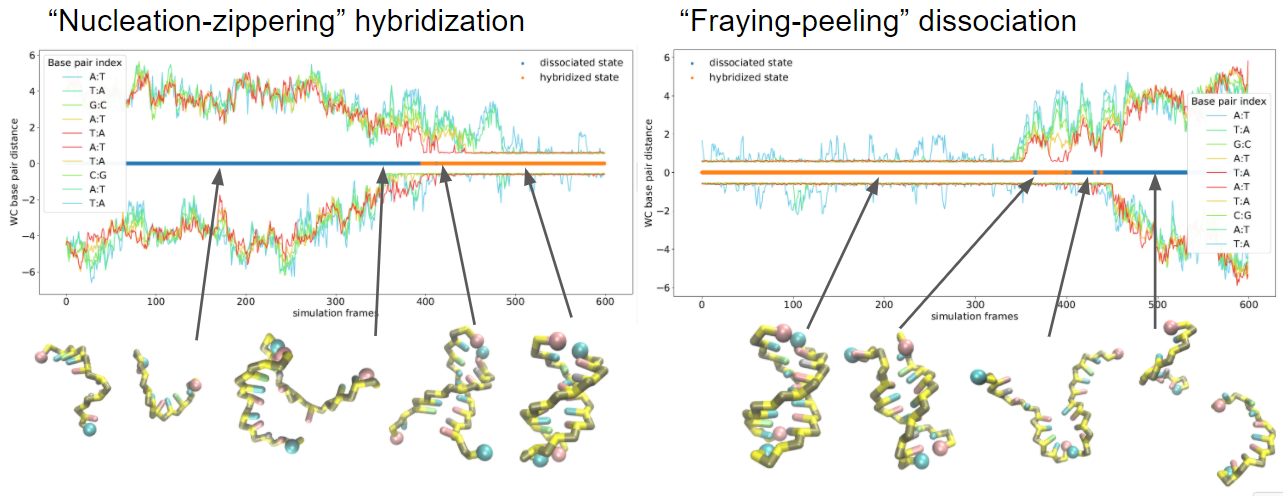
\includegraphics[width=\textwidth]{Figs/figs_imp/GC-mix_transitions.PNG}
        \caption{WC base pair distance and molecular renderings along two representative GC-mix hybridization and dissociation events.}
        \label{fig:GC-mix_transitions}
	\end{center}
\end{figure}


%%%%%%% start of "interesting phenomena" section   %%%%% 
\subsection{Diffusion maps show structural diversity within PCCA+ macrostates}

% add new diffusion map section introduction
Although our SRV-MSMs provide useful insight into slow processes, we are also interested in the ensemble of configurations within PCCA+ macrostates. These configurations interchange significantly faster than the SRV and MSM lag times, but we can use a diffusion map embedding to glean a structural understanding of the macrostate population. Diffusion maps generate a low dimensional embedding of the data into high variance structural modes and are well-suited to find subtle differences in temporally disconnected data \citep{Coifman2006DiffusionMaps, Ferguson2010SystematicMaps}. We were particularly interested in using this method to explore the 5s1 and F4 macrostates as these represent the most popluated and kinetically relevant macrostates for AT-all, GC-end, and GC-core.

% use this to substantiate the shifted fast response
\subsubsection{5s1 state analysis}
While examining molecular renderings, we noticed that a significant proportion of GC-end 5s1 configurations retained one native G:C bond, even when all available A:T bonds were formed out-of-register. We would not necessarily expect duplexes to sacrifice helical conformational entropy in order to facilitate termini bonding. To compare how these state populations differ between GC-end and AT-all, we employed diffusion maps built on an equal sampling of 5000 conformations from the 5S1 state of both sequences. We used all 100 intermolecular distances (as opposed to the 55 permutation free coordinates used to construct SRV-MSM) as our distance metric, making it easier to discern structures that form on either permutable end of the shifted conformation. This created a degenerate 2nd and 3rd diffusion modes, with nearly equal eigenvalues, differentiating between looping at the identical "top" and "bottom" of the strands. In Figure \ref{fig:GC-end_dmaps} we present the first two non-trivial diffusion map eigenfunctions and show representations of the degenerate third coordinate in the SI (Figure \ref{fig:GC-end_dmaps_full}). Diffusion maps built from samples of the 3' shifted states are also shown in the SI (Figure \ref{fig:GC-end_dmaps_3prime}). 

The first diffusion mode clearly delineates between the GC-end and AT-all shifted conformations and correlates highly with the average distance between the 3' end and its shifted complementary pair. This reveals that the mismatch C:T-pairs are never bound -- a consequence of the 3spn2 excluded volume interaction -- whereas the AT-all pairs are mostly bound with occasional fraying indicated by small AT-all overlap in the GC-end region. This effect may be exaggerated given that C and T base pairs are assigned slightly higher excluded volume radii in 3spn2 \citep{Hinckley2013AnHybridization}. The second diffusion mode, which correlates highly with the average distance between 3' and 5' ends, has higher values for GC-end than AT-all. Because the GC-end termini do not bind out of register, we find that they are readily able to form stabilizing contacts despite the shifted conformation of the duplex as a whole. These "shifted-loop" bonds are shown to be uniquely stable for GC-end conformations in the 5' shifted state, and their existence in the simulations confirmed by molecular renderings of these regions Although AT-all shifted ends tend to stay bound out-of-register, the second diffusion coordinate shows some population of inert tails that fold back onto the helix.

% need to work on this if adding to this section (might belong somewhere else or not at all?
Although internal base pair mismatches can cause substantial conformational distortions such as kinking, terminal mismatches have been shown to be slightly stabilizing and have a minimal effect on helical character \citep{Santalucia2004TM, DiMichele2014EffectHybridization}. In the context of the 3spn2 model, these ends are accounted for via intra-strand base stacking and inter-strand cross-stacking interactions \citep{Hinckley2013AnHybridization}. The only direct interaction between non Watson-Crick (WC) basepairs is parameterized by isotropic excluded volume potential, which is likely more simplistic than the true mismatch interaction. 

%AT-all looping could be a consequence of multiple bps sharing the same wc partner (I believe this is possible in 3spn2, because types of bonds are only mutually exclusive between cross-stacking, bp binding, and excluded volume)%

\begin{figure}[ht!]
	\begin{center}
        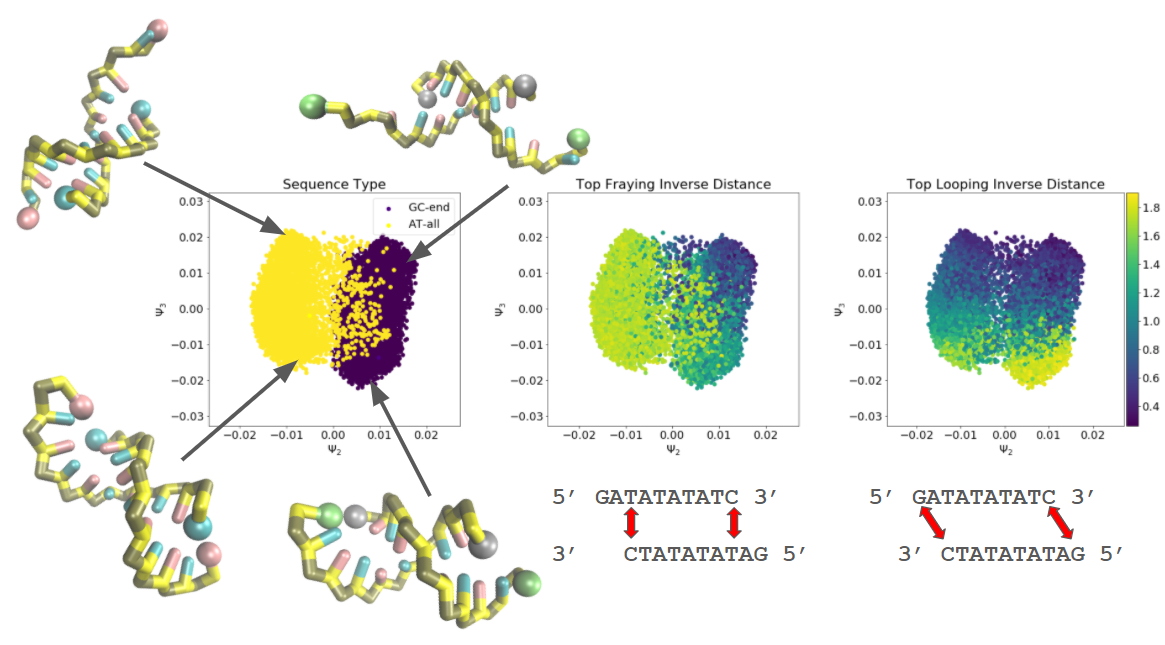
\includegraphics[width=\textwidth]{Figs/figs_imp/GC-end_dmaps.PNG}
        \caption{First two diffusion map coordinates built from 10000 5S1 states, equally sampled from AT-all and GC-end. Color maps show inverse distances between out-of-register ends and complementary ends.}
        \label{fig:GC-end_dmaps}
	\end{center}
\end{figure}


\subsubsection{F4 state analysis}  % shift to include this in the overall diffusion map section
%\subsubsection{Diffusion maps show ensemble of frayed states}

We applied a similar approach to investigate the structural composition of the F4 macrostate. We build diffusion maps using 10000 frames sampled from the macrostate \ref{fig:GC-core_dmaps}. This time, we set our distance metric to the same permutation-free coordinates we used to build the SRV-MSMs. Again, we were able to identify a combination of physical coordinates that closely correlated to the first two non-trivial diffusion modes. We found that a larger distance between the third and fourth A:T pairs increased the PCCA+ probability of inclusion into macrostate. This distance also correlated closely with the second diffusion map mode. Interestingly, we observed that the first non-trivial mode -- the feature that describes the most structural diversity in the system -- corresponds to difference in "overlap" distance between adjacent A or T bases and the GC core. In these conformations, one of the strands maintains some helical character while the other twist out of place, resulting in WC bonds being obstructed by the oligo backbone. These states represent another potential way in which the hybridization process (or helix reformation) can be kinetically frustrated. We observed this mode to be mostly symmetric, however there is slight tendency for the 3'T end to fray farther out of place relative to its 5'A counterpart. This might be another consequence of differential excluded volume radii in the 3spn2 force field.

\begin{figure}[ht!]
	\begin{center}
        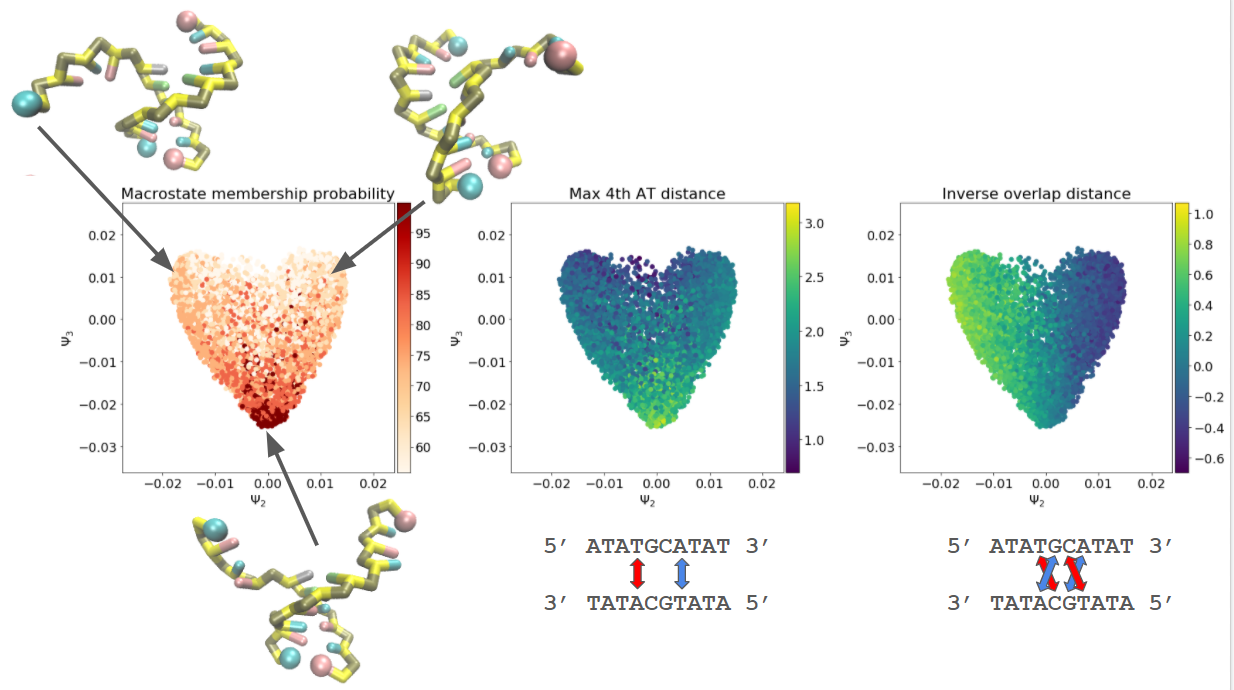
\includegraphics[width=\textwidth]{Figs/figs_imp/GC-core_dmaps.png}
        \caption{Plotting the first two non-trivial diffusion map eigenfunctions. Color maps show the probability that conformations are clustered into the frayed macrostate, maximum distance between 4th AT basepairs, and the the overlap between adjacent AT basepairs and the GC core.}
        \label{fig:GC-core_dmaps}
	\end{center}
\end{figure}


% not sure if this should directly follow the SRV-MSM GC-core description or directly follow the GC-core dmaps?
\subsection{SRV correlations to physical coordinates}

Having constructed and interpreted SRV-MSMs, we revisited our original SRV basis to investigate how slow modes are constructed from input features. We found these GC-core modes to be of particular interest as they reveal the hierarchical and nonlinear nature of the dynamical encoding. In particular, we examined a collection of "trimmed" trajectories centered on both hybridization or dissociation events. For each trajectory, we compared the first three SRV coordinates with a corresponding collective variables with which they shared behavior. Two representative trajectories are shown in figure: (\ref{fig:GC-core_tracking_modes}). Complementary G:C pairs are the best indicators for a hybridization/dissociation event, and we see a sharp change in the first SRV mode (SRV1) as these bonds form or break. The second slow mode (SRV2) is most active when G:C pairs are bound but the adjacent AT pairs are not. There is a small signal for fraying at the outer base pairs, but the mode overwhelmingly learns about these neighboring A:T/G:C bonds. This behavior reflects movement in and out of the F4 state in the corresponding SRV-MSM. SRV3 is most active during dissociation, and seems to track closely with the average distance between all complementary base pairs. We attribute this to the SRV learning about the diffusive motions of the two body system and evaluating the likelihood of an imminent hybridization event. The third mode also peaks when the oligos are close together but configured in such a way that is not amenable hybridization. These misaligned conformations include inverse contacts where 5'/5' and 3'/3' ends meet and looped conformations where one strand is folded in on itself and preventing satisfactory WC contacts. 

Despite the strong trends we observe between physical coordinates and leading SRV modes, we only find high Pearson correlations between SRV1 and physical coordinates. For the next two SRV modes, the sign of their correlation switches depending on whether the oligos are in the hybridized or dissociated state. This shows that these modes are providing support on top of the first mode -- which serves as an indicator function for hybridized vs. dissociated state -- and thus can display very different behavior in either state. With respect to our SRV-MSM macroscates, we found that SRV2 was "turned on" in the H and F4 states -- corresponding to the intact helix and frayed state, respectively -- and SRV3 was turned on in the dissociated state. Accordingly, we calculated Pearson correlations between each SRV mode and all distances in states where the modes are active. Figure \label{fig:GC-core_tracking_modes} shows the highest correlation between SRV2 and inner A:T pairs, weak correlation with outer A:T pairs, and an inverse correlation with 5'/5' and 3'/3' pairs which tend to approach each when the duplex is in the F4 state. We also observed a highly symmetric correlation between SRV3 and central base pairs distances, which indicative of overall diffusive behavior. Taken together, these analyses reveal how the SRV learns and represents the dynamical space in an hierarchical manner, providing enhanced resolution to a linear method like tICA and producing the MSM results we observe above.

% note that similar analysis on AT-all and GC-end can be found in the SI (move both dynamics plots and descriptions there)

\begin{figure} %[ht!]
	\begin{center}
        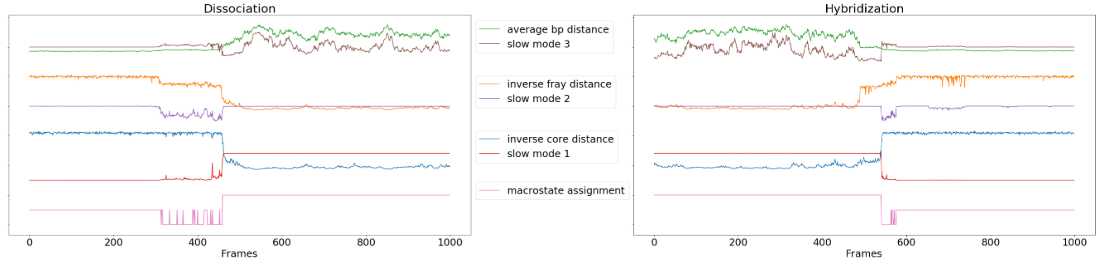
\includegraphics[width=120mm]{Figs/figs_imp/GC-core_tracking_modes.png}
        \caption{Leading GC-core SRV coordinates correlated with identifiable physical coordinates during sample hybridization (a) and dissociation (b) events. (c) Pearson correlations between all 100 intermolecular base pair distances and each the three leading slow modes. SRV2 correlations were calculated in the H and F4 states; SRV correlations were calculated in the D state.}
        \label{fig:GC-core_tracking_modes}
	\end{center}
\end{figure}    


\subsection{\label{sec:Results}Temperature-dependent timescale comparisons}

Given differences in temperature and ensemble distributions between Tmelt simulations and T-jump experiments, we found it difficult to make direct timescales comparisons based on our equilibrium models alone. To supplement our analysis, we ran short simulations initialized in the hybridized state at a series of elevated temperatures for each sequence. We derived relaxation times for a "slow" dissociation response and "fast" fraying response at each temperature and compared these with experimental temperature-dependent relaxation fits for GC-end and GC-core. Additionally, we repeated the protocol in Sandstead et al. to generate temperature series data for AT-all and GC-mix sequences \citep{Sanstead2018DirectDehybridization}. 

We measured the slow dissociation response by fitting the distribution of times at which the core base pairs separate beyond a cutoff. We found the inverse of these relaxation times -- the effective dissociation rate -- to increase exponentially with temperature, which is expected given the large enthalpic barrier of dissociation. Furthermore, we see an acceleration of about one order of magnitude compared to experiment, although this factor is sensitive to the exact definition of melting temperature which can vary between simulation experiments. After accounting for the acceleration factor, we saw agreement between the experimental data and simulated relaxation fits. GC-core showed the largest deviation experiment, with dissociation rate increasing much more quickly with temperature in simulations.

% GC-core fast timescales could be slower as they have contributions from internal fraying which would have a longer relaxation than the termini alone.
% in order to make comparisons across these different free energy landscapes, we adjusted simulations by a consistent acceleration factor. We maintained a consistent accerelation factor across sequences, but found that optical scaling different by about one order of magnitude between fast and slow responses. It is expected given that different degrees of freedom often experience differing amounts of accelerations in coarse-grained models.

\begin{figure}  %[ht!]
	\begin{center}
        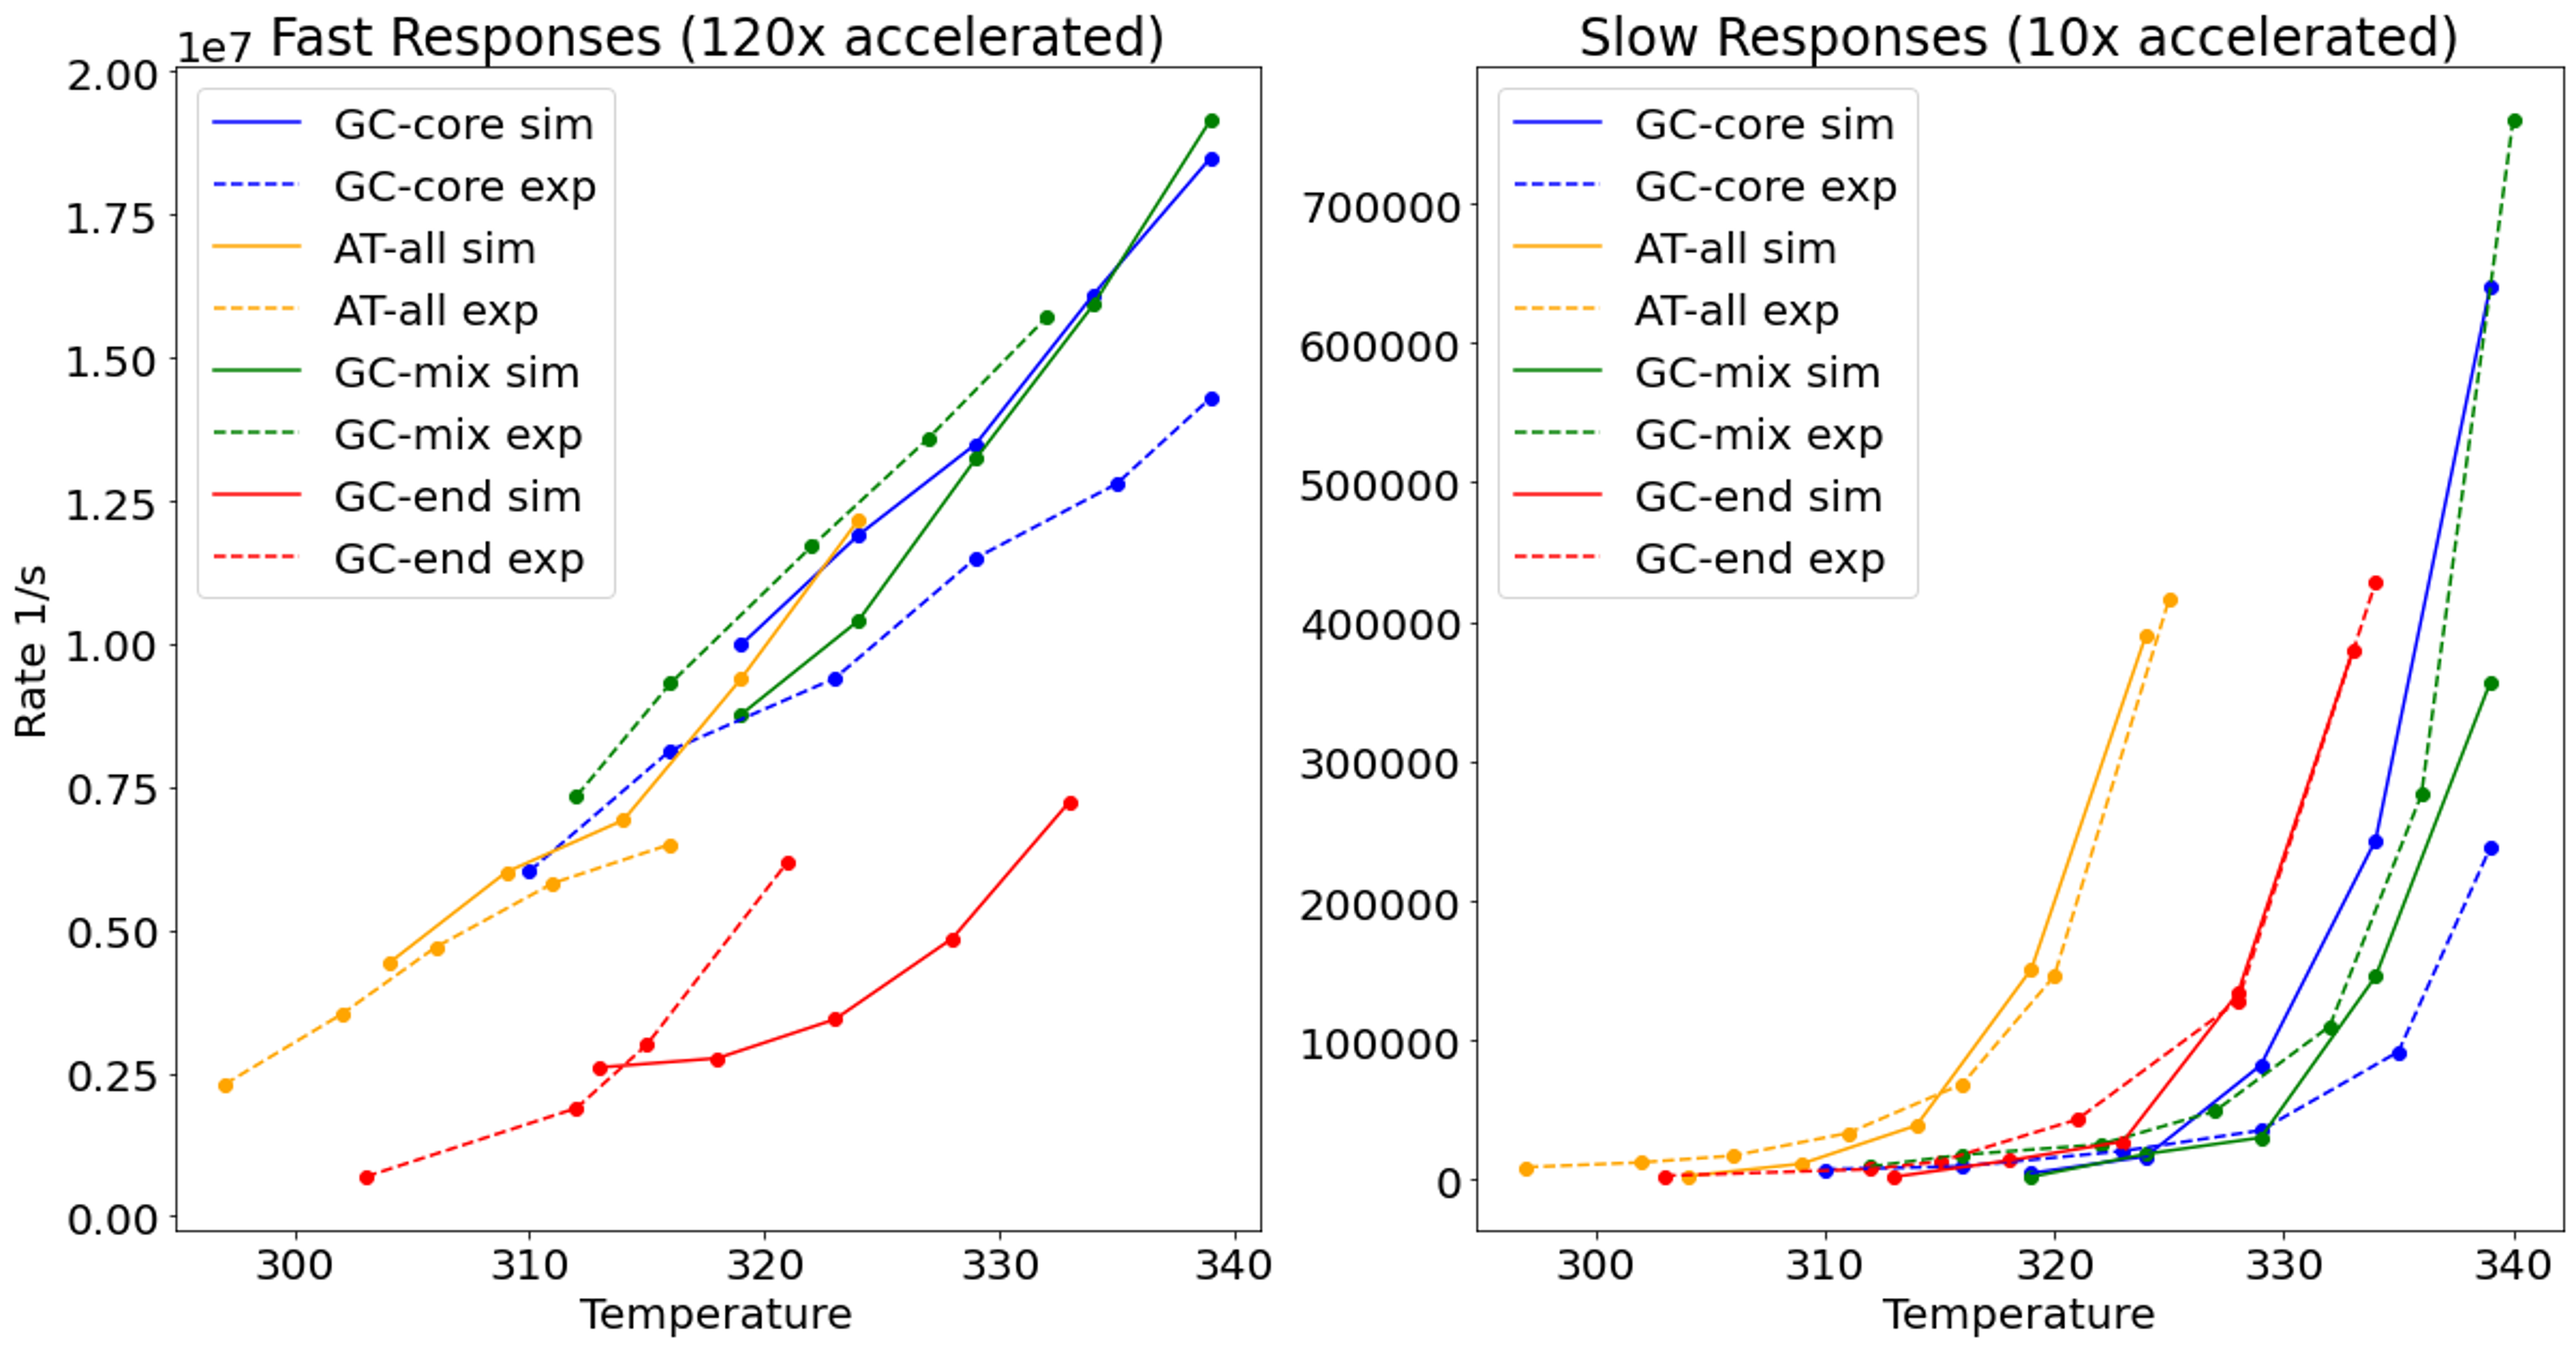
\includegraphics[width=\textwidth]{Figs/figs_imp/Tjump_responses.png}
        \caption{Fitting temperature-dependent trends to the "slow" dissociation mode and "fast" fraying mode detected in experiments. The effective simulation temperature is shifted by 4 degrees K to account for systematic differences in simulation and experimental melting temperature. Different scaling factors are applied to fast and response to account for variable coarse-grained acceleration along different degrees of freedom.}
        \label{fig:relaxation-comparison}
	\end{center}
\end{figure}

% A documented short-coming for the 3spn2 model is a high proclivity for termini fraying relative to what has been observed in vitro \citep{2013}. This supports why we observe significantly more acceleration for the fast response, but relative sequence and temperature effects still compare well with T-jump results.

The fast response -- which Sanstead et. al attributed to base pair fraying signatures -- was more difficult to compare against simulation observables. Numerous experimental and computational studies have shown that DNA and RNA fraying is a complex dynamical process with timescales that span 5 ps to several microseconds \citep{ Nonin1995TerminalFraying, Nikolova2012ProbingSimulations, Andreatta2006UltrafastHelix, Galindo-Murillo2015ConvergenceDGCACGAACGAACGAACGC}. All-atom simulations suggest that frayed ends can assume misaligned WC bonds, base-sugar hydrogen bonds, and terminal stacked conformations \citep{PinamontiTheModels, Zgarbova2014BaseRNA}. Given that there is only one interaction site parameterized on each 3spn2 base, we would not expect to resolve this diverse collection of states and dynamics. Instead, we measured the fast fraying response by counting frames until either duplex terminal end to split beyond a cutoff. This approach assumes that fraying on the permutable top and bottom of the duplex are independent from each other, and that a base pair distance is a reliable approximation for the ensemble spectroscopy signal. This is a reasonable assumption given that the amplitude-weighted timescales should consist largely of terminal fraying events. Again we fit relaxation curves to the ensemble of fraying timescales in order to extract rate approximations for each sequence at a series of temperatures. Experimental comparisons at high temperatures were limited due to mixing between the fast and slow responses.

For A:T terminal sequences, the simulated fast response appears linear with temperature, indicating a barrierless and diffusion-driven process. In contrast, the GC-end responses are distinctly slower and increase exponentially with temperature, likely due to a greater thermodynamic barrier associated with G:C fraying. We observe similar trends in the experimental data, especially after applying a consistent acceleration factor as shown in figure \ref{fig:relaxation-comparison}. We found the optimal acceleration factor to be dependent on the choice of the cutoff parameter, but we can approximate that 3spn2 fraying dynamics are accelerated by about two order of magnitude relative to experiments. It is not surprising that we see different rates of acceleration for the dissociation and fraying processes given that coarse-grained effects can vary across different degrees of freedom. In particular, the simplified treatment of the fraying process may smoothen the free energy landscape and speed up dynamics relative to a more global processes like dissociation. Although we should rely on higher resolution models to study in depth mechanisms of fraying, our results indicate that terminal fraying is a reasonable assignment for the spectroscopic fast response in Sanstead et al. and that 3spn2 can capture some sequence-dependent fraying effects.

%Again, GC-core behavior deviates from simulations prediction with consistently lower than expected fast responses. We believe this could be due to slower contributions from internal A:T base pairs sequentially fraying. 

% Experiments fast responses are difficult to discern at higher temperatures due to mixing with slow responses. This is especially true for GC-end because to the signals are closer to begin with.
% add new info here, not sure if shifting discussion is necessary
% take away message is that these are good proxies for the responses
% although there is not perfect agreement, we show that these are very reasonable coordinates assing fast and slow response

%In addition to fraying, we notice that the rate of shifting increases at higher temperature. Moreover, the thermodynamic stability of these shifted conformations increases relative to that of intact duplex. For T-jumps at higher initial and final temperatures, it is possible that some portion of the starting ensemble is in a shifted state and that the fast dynamics are increasingly influenced by alternative "looping" G:C bonding that we observed in our diffusion map analysis above. It is less likely that shifting mechanisms would have their own distinct signals, given that these occur at far lower frequency than fraying or full-dissociation, but we believe that further experimental work is necessary to investigate this phenomenon.

%The temperature-dependent analysis can also inform out interpretation of the 3spn2 model. Previous work has shows that kinetic association rates were accelerated by about one to two orders of magnitude relative to experiment \citep{Hinckley2013AnHybridization}.  It is not surprising that different dynamics might be accelerated at different rates, especially considering that 3spn2 was not extensively parameterized on dynamical properties properties \citep{Hinckley2013AnHybridization}. 

%We also did not find available data on other acceleration studies using explicit ions.

\section{\label{sec:conc}Conclusion}

We have demonstrated how coarse-grained MD can be supplemented by data-driven time-lagged analysis to efficiently learn the slowest processes of DNA hybridization. We constructed high resolution SRV-MSMs capable of distinguishing sequence-dependent dynamics, and showed the relevance of these dynamics to experimental results. We found that AT-all and GC-end sequences both participate in some degree of out-of-register base pair shifting, although these states have higher kinetic relevance for AT-all. On the other hand, GC-core hybridization transits through, or is perhaps facilitated by, a frayed intermediate in which one half of A:T bonds are broken and the duplex is significantly disrupted. This approach allowed us to aggregate an ensemble of trajectories in order to properly sample hybridization and dissociation without bearing a large computational expense. Furthermore, we replicated T-jump analysis across a series of temperatures to verify previous spectroscopic assignments and sequence-dependent effects at different timescales.

\subsection{\label{sec:conc}Limitations} 

Although we were able to obtain improved resolutions on several relevant dynamics by using a shared lag time across sequences, we found it difficult to converge on relevant faster processes such as duplex nucleation and zippering. These processes are crucial to duplex formation, however they do not appear to be kinetically metastable or slow relative to other timescales of interest. Furthermore, they can initiate at various points along the strand, which, under out present featurization method, may appear as a collection of modes instead of as one distinct process. We also found the need to strike a balance between adequate sampling of hybridization events and frame save rate in order to maintain tractable SRV-MSM calculations. Indeed, we collected over 10 GB of equilibrium trajectory data for each sequence, and were working near memory limits when training SRVs and building SRV-MSMs.

In any high-level model there are inevitable simulation artefacts produced by coarse-grained approximations. For example, the treatment of non-interacting base pairs as an excluded volume potential alone may not be representative of dynamics produced from mismatched dangling ends. In general, coarse-grained models produce a smoother free-energy surface which can results in must faster motions between states. This is illustrated by substantial accelerations in temperature-dependent responses when compared to experiment. Furthermore, it may be easier to cross between states -- e.g. a 5S1 $\rightarrow$ H transition -- when the usually rough free energy path becomes more easily traversed. 

\subsubsection{\label{sec:conc}Not sure whether to discuss explicit comparisons} 
We also acknowledge that the implicit model may not fully capture the role of ions in facilitating hybridization and dissociation. In addition to implicit simulations, we followed the same pipeline to generate simulations and SRV-MSMs given the exact ion conditions specified in the \citet{Sanstead2016} using the 3spn2 explicit implementation \citep{Hinckley2015}. These results look very similar to the implicit case, although with slightly slower dynamics and higher uncertainty in stationary probabilities. Comparisons were limited by the higher computational demand required to simulate 5x the beads in the box, a shorter integration timestep, and reliance on Ewald summation to account for electrostatics. We caution over-interpretation of these results as the explicit model has not been as widely adopted or thoroughly validated compared to the implicit model.

(Should add something else here or re-arrange above...) Going forward, we believe that this work will contribute novel insights to DNA design strategies, and can be leveraged as a prediction mechanism for the broader sequences spaces.


\section{\label{sec:Results}SI Methods notes}

% add secion on dmap and high temp methods?
%\subsection{Additional methods}

%In order to maximize concentration without allowing strands to see each other through periodic boundaries, we set the box size just larger than the sum of the maximum end-to-end extension length of a single strand and the force cutoff.



\subsubsection{SRV optimization and analysis}
In our analysis, we found that the AT-all sequence, given its repetitive structure and lack of GC-content, produced the simplest dynamics and displayed a clear spectral gap between modes. For this reason, we use this sequence a case study to work through our SRV-MSM pipeline step-by-step. Our first task was to identify the SRV lag time that was longer than the intrinsic Markov timescales of the system, yet short enough to resolve the dynamics of interest \citep{Phys2018MarkovValidation}. We found that most implied timescales converge at an SRV lag time of 1.2 ns. Next we selected an optimal number of SRV components to include in our analysis. After a certain point, higher order dynamical modes provide diminishing contributions the overall kinetic variance as measured by the Vamp-2 score, and the model can begin fitting on statistical noise in the trajectory data instead of the true dynamics \citep{McGibbon2015VariationalKinetics}. It is also more difficult to perform kmeans clustering on a high dimensional space, especially when those higher dimensions are less kinetically relevant \citep{Pande2010EverythingAsk}. For these reasons, the number of slow SRV components should be carefully selected based on the specific system of interest. As shown in figure \ref{fig:allseq_srv_crossval}), we see diminishing returns in the VAMP-2 score after five slow modes and select these modes as our optimized SRV basis.

%\subsubsection{SRV-MSM construction and optimization}
Although SRV coordinates alone provide some information, we can access a more holistic picture of sequence kinetics and thermodynamics by using these SRV coordinates as a basis on which to construct an MSM. Because these coordinates are already capturing a majority of the system's kinetic variance, they serve as an ideal basis on which to group frames into microstates. We performed k-means clustering, and optimized the number of microstates at 200 by monitoring VAMP-2 score. Next, we selected an MSM lag time in a similar fashion to our SRV lag time selection process. This enables us to select a shorter lag time and build a higher resolution model than we could from an analogous tICA basis. Setting the MSM lag time to the same 1.2 ns we used for our SRVs, we built a Bayesian MSM to calculate transition probability matrix between each microstate. Finally, PCCA+ spectral clustering was implemented to group these microstates into macrostates that each represented a collection of metastable structures. Previous works have used a common set of microstates and/or performed manual clustering of microstates based on physical read outs from simulation data (stacking score, energies, etc) \citep{Pinamonti2017PredictingModels, PinamontiTheModels}. Although these techniques are useful for performing comparisons between sequences, we saw better results when optimizing MSMs to capture the most detail of sequence individually and thus developed an independent set of microstates and macrostates for each sequence. 

Next, we seek to interpret the physical relevance of these leading modes by plotting the Pearson correlation of each mode with the 100 intermolecular distances between strands. The quantitative meaning of these coordinates can be difficult to interpret given their nonlinear relationship to the SRV collective variables, but the relative different between these correlations shows which coordinates are most relevant to each process. For example, the first slow mode shows a positive correlation to each distance and the strongest correlation with native base pair distances (shown along the main diagonal). Given these correlations and the substantially longer timescale of this process, we can deduce that this leading mode corresponds to the overall hybridization and dissociation process. The next four SRV components all show a relatively high correlation along offset diagonals. These diagonals correspond to the intermolecular distances between complementary but out-of-register base pairs and point to the existence higher order "shifting" processes between sets of such base pairings. Previous "inchworm" and "pseudoknot" mechanisms have similarly been reported in simulation studies to correct base pair mismatches and occur on orders of magnitude longer timescales than underlying fast dynamics such as fraying \citep{Romano2013DNADependence, Markegard2015, Maciejczyk2014DNAModel}.

We found GC-end had a similar implied timescales distribution to AT-all, with a distinct spectral gap after the fourth mode. For AT-all and GC-end, we kept to the convention of clustering into n+1 macrostates, where n is the number of slow components captured by the MSMs. For GC-core we built an SRV-MSM using these first three SRV modes as a basis and proceeded along the pipeline as described above. We found that four macrostate clustering was unstable -- likely because the third mode is mostly providing  information about dissociation dynamics -- so we performed PCCA+ clustering into three macrostates representing the hybridized (H), dissociated (D), and 4 4 base pair frayed (F4) states.  The GC-mix sequence showed a similar implied timescale distribution to GC-core, however we no longer saw a converged slow mode corresponding to multi-base fraying behavior. Instead, we observed two modes converge, corresponding to the association/dissociation dynamic and diffusive behavior while strands are dissociated. These correlate closely with the first and third GC-core SRV modes. Although we built our SRV-MSM using these two coordinates, we again were unable to form a stable third state along the second coordinate. As such, we designated this transitions as effectively two-state within the resolution of our model.

%For GC-core and GC-mix, we found this clustering convention to be unstable -- likely because the last converged mode was providing information about dissociation dynamics -- and performed PCCA+ with one less macrostate. 

To visualize macrostates, we project the data into the two leading tICA coordinates. Although SRVs outperform these coordinates for the purpose of MSM construction, tICA coordinates represent good high variance collective variables on which to visualize free energies and state assignments \citep{Sidky}. Furthermore, we found that all macrostate were discernable on the first two tICA coordinates, whereas multiple SRV dimensions would be necessary to visualize states. After assigning these macrostates we calculated their stationary and transition probabilities averaged across 100 Gibbs sampled MSM and PCCA+ assignment. Means and standard deviations were calculated from this ensemble.




\subsection{\label{sec:Results}SI figs}

\begin{figure}[ht!]
	\begin{center}
        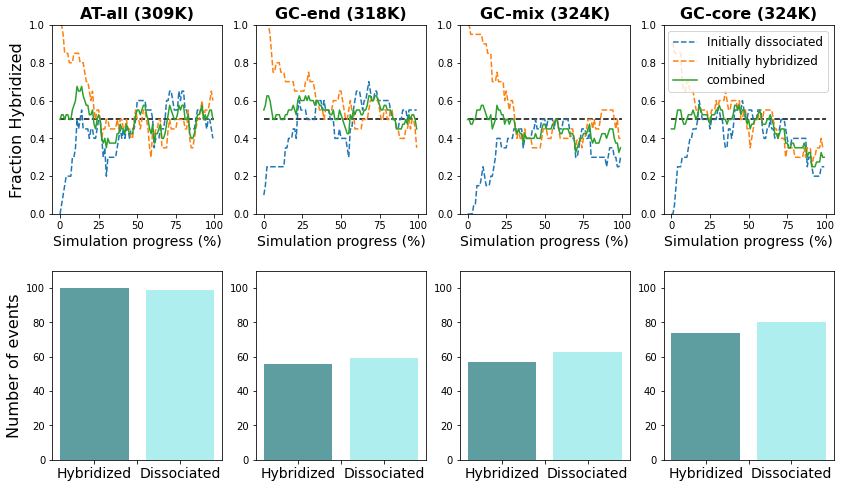
\includegraphics[width=120mm, 
        scale=0.5]{Figs/figs_imp/allseq_event_count.png}
        \caption{All sequences consist of 20 trajectories initialized in the hybridized states and 20 in dissociated state. The fraction of hybridized duplexes averaged across these sets is shown over time. For all sequences these curves converge near 0.5, but stochasticity of rare-event makes a definitive Tmelt difficult to identify. The number of hybridization/dissocation combined across trajectories is shown. Not every trajectory contained a transition event, but on average more than one full event occurred (H$\rightarrow$D$\rightarrow$H) per trajectory, providing adequate sampling of dynamics. AT-all undergoes substantially more transition, but many of these do not reach a native (in-register) hybridized state.}
        \label{fig:allseq_event_count}
	\end{center}
\end{figure}

\begin{figure}[ht!]
	\begin{center}
        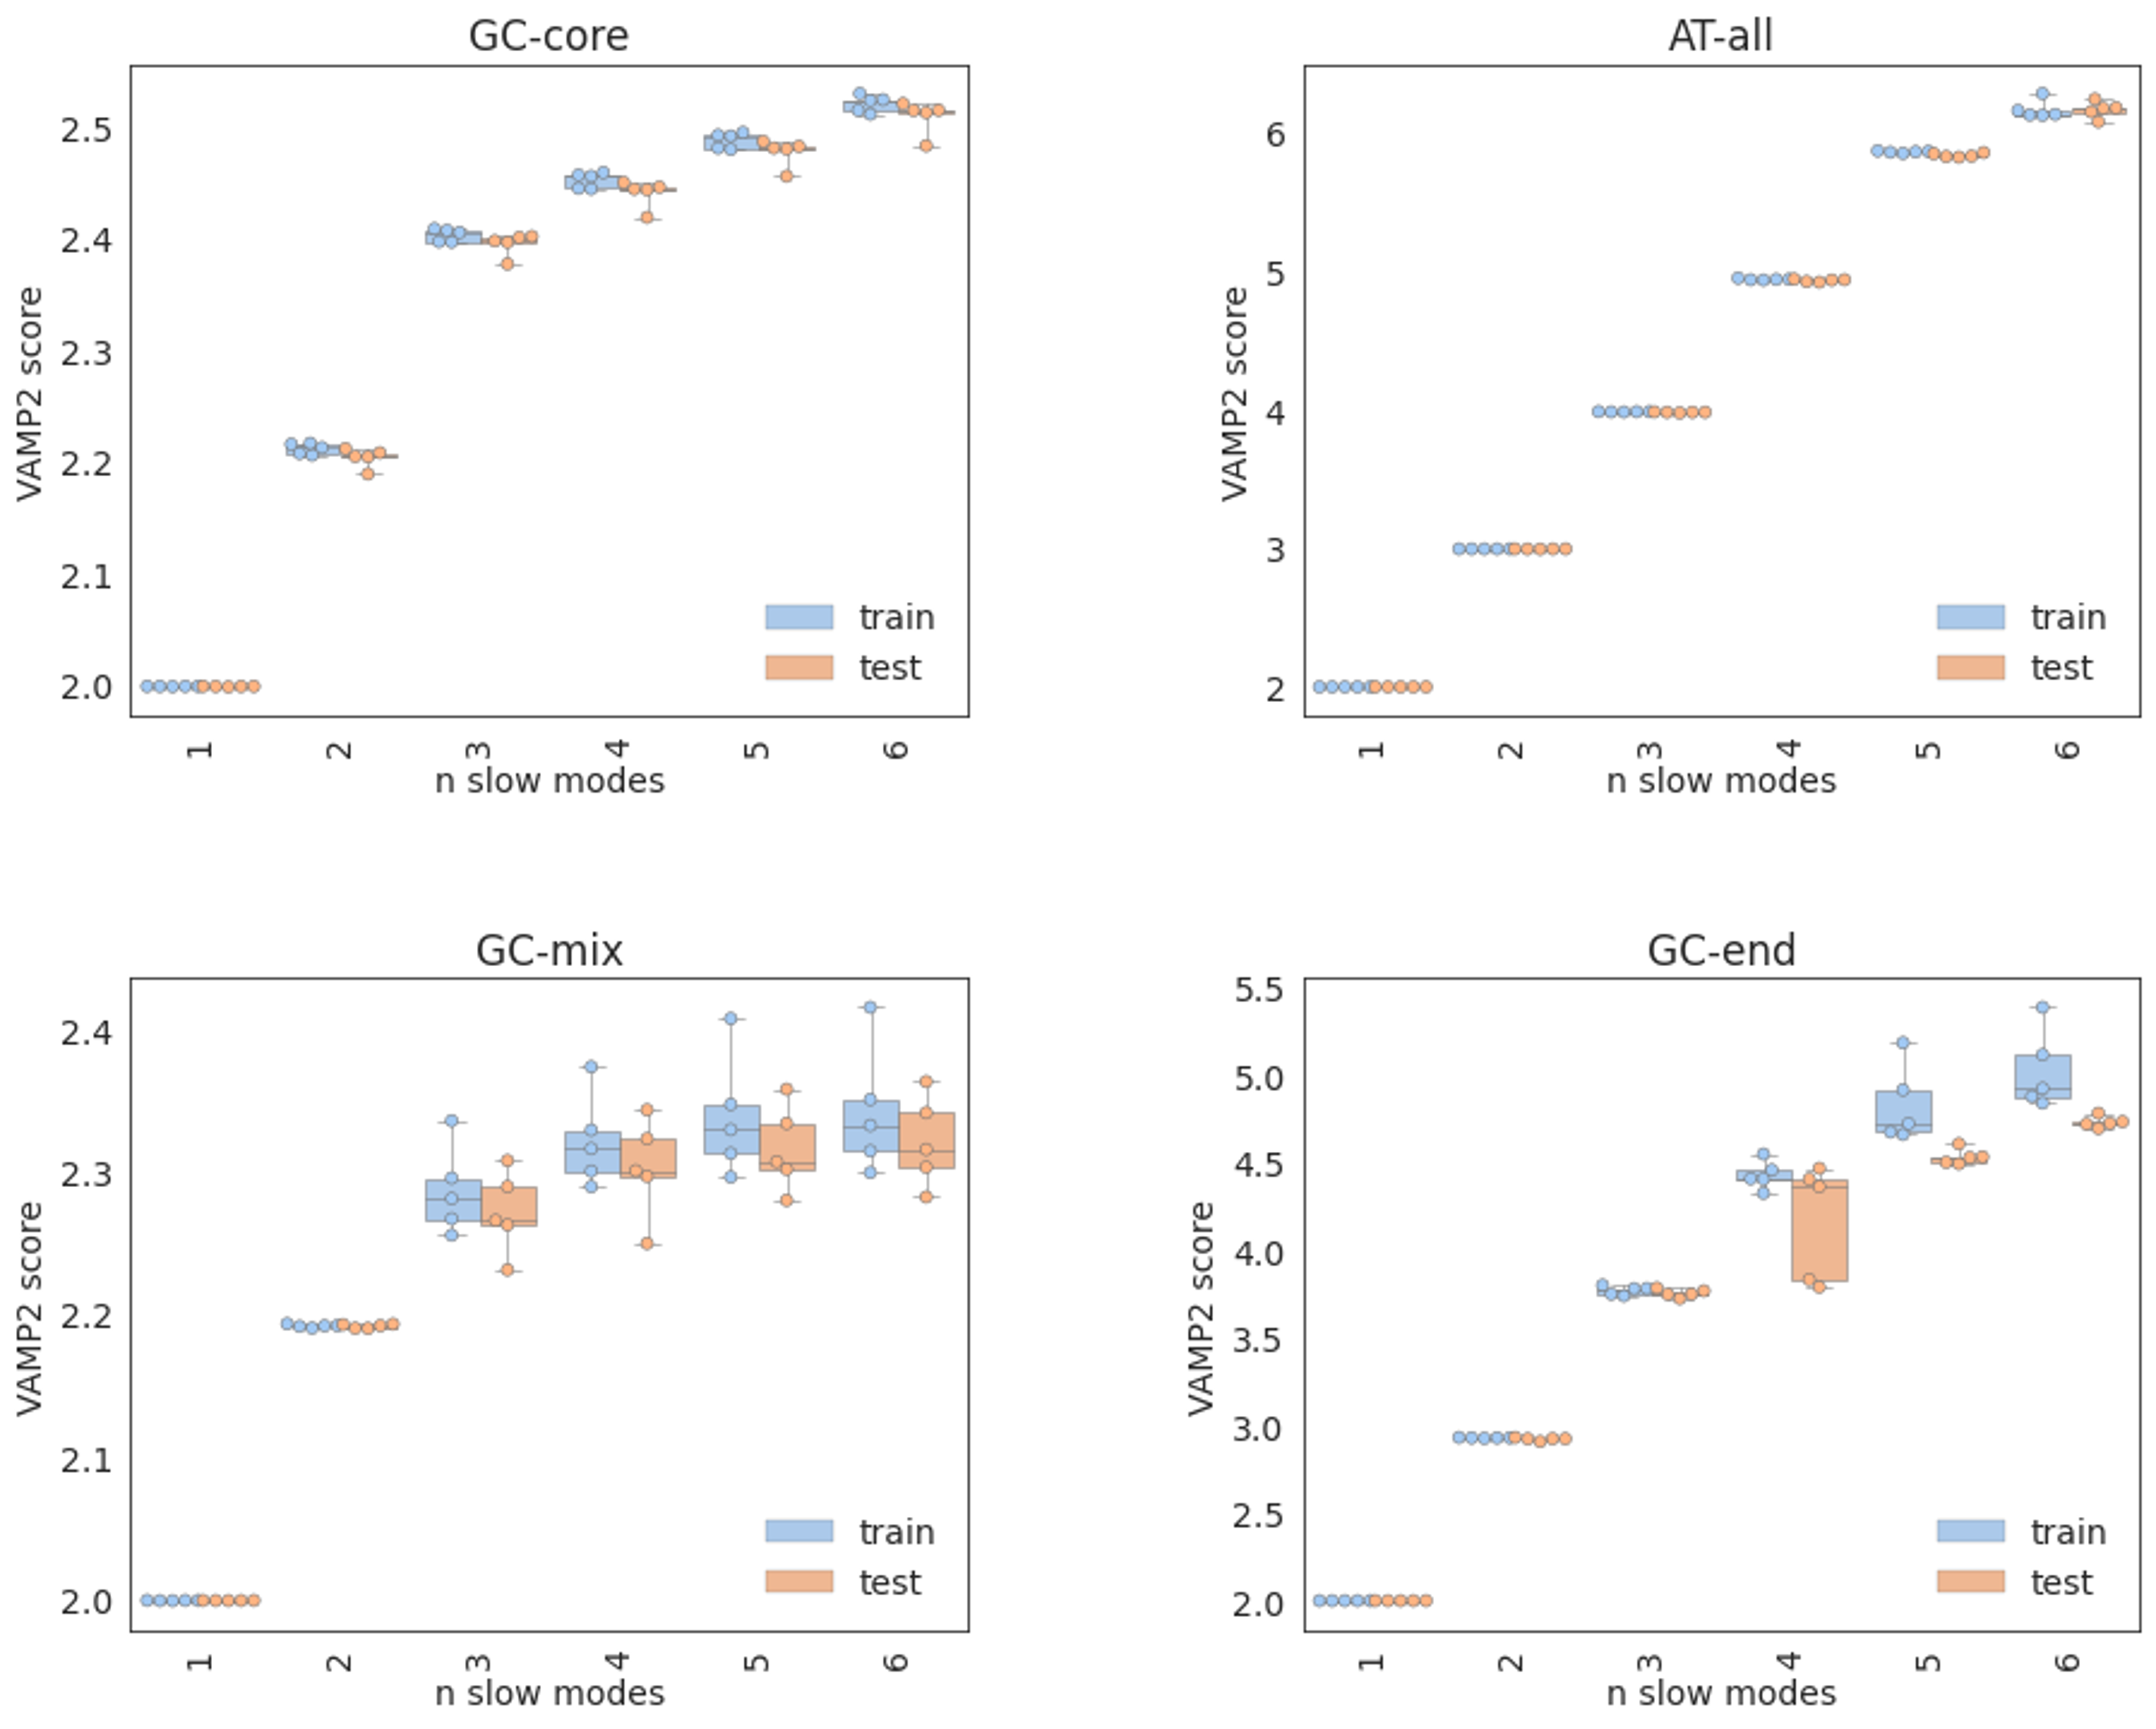
\includegraphics[width=120mm, 
        scale=0.5]{Figs/figs_imp/allseq_crossval.png}
        \caption{5-fold cross validation procedure to select number of SRV coordinates. We look for the converge of the VAMP-2 scores, inconsistent scores between folds, and deviation between training and test data as indicators that the model has begun fitting on statistical noise.}
        \label{fig:allseq_srv_crossval}
	\end{center}
\end{figure}

\begin{figure}[ht!]
	\begin{center}
        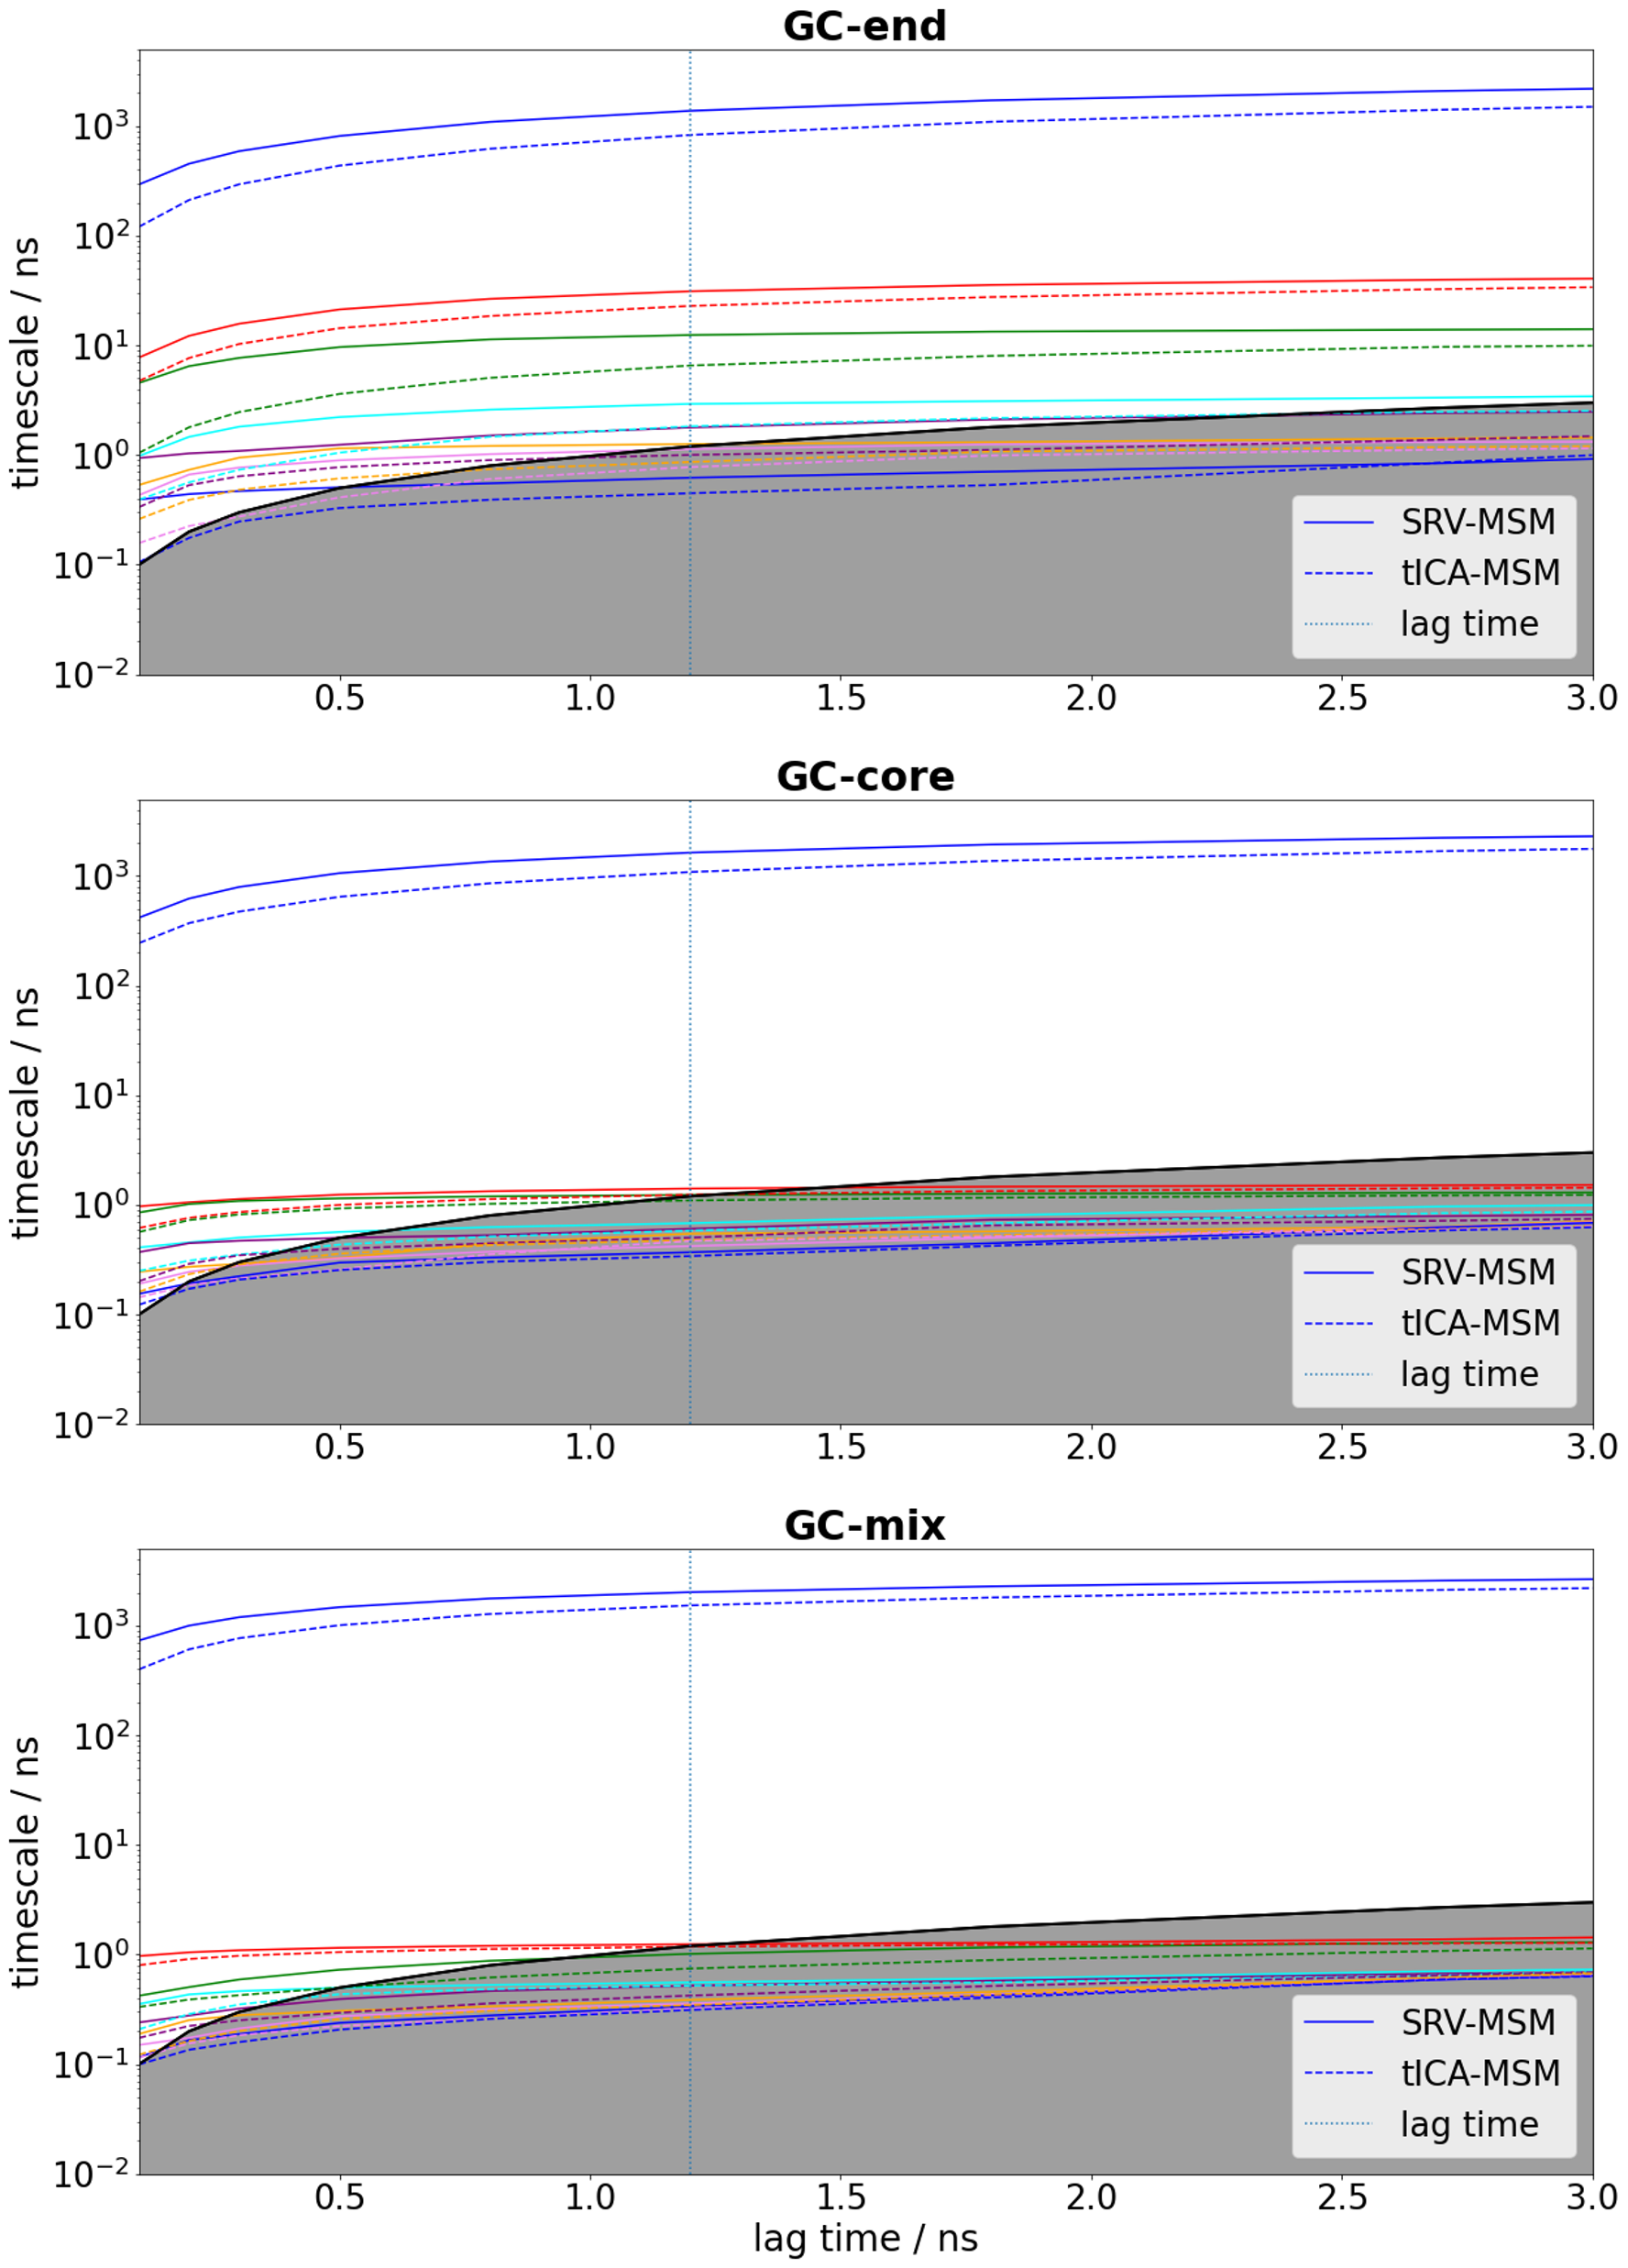
\includegraphics[width=80mm, 
        scale=0.5]{Figs/figs_imp/all_seq_implied_times.png}
        \caption{SRV-MSM vs. tICA-MSM implied timescales convergence for GC-end, GC-core, and GC-mix. Progressively larger spectral gaps are observed between the first mode and higher order modes. We observe convegenve of resolvable higher order modes at a shared lag time of 1.2 ns. It is difficult to converge the leading mode in this regime due to the infrequency of hybridization/dissociation events.}
        \label{fig:all_seq_lags}
	\end{center}
\end{figure}

\begin{figure}[ht!]
	\begin{center}
        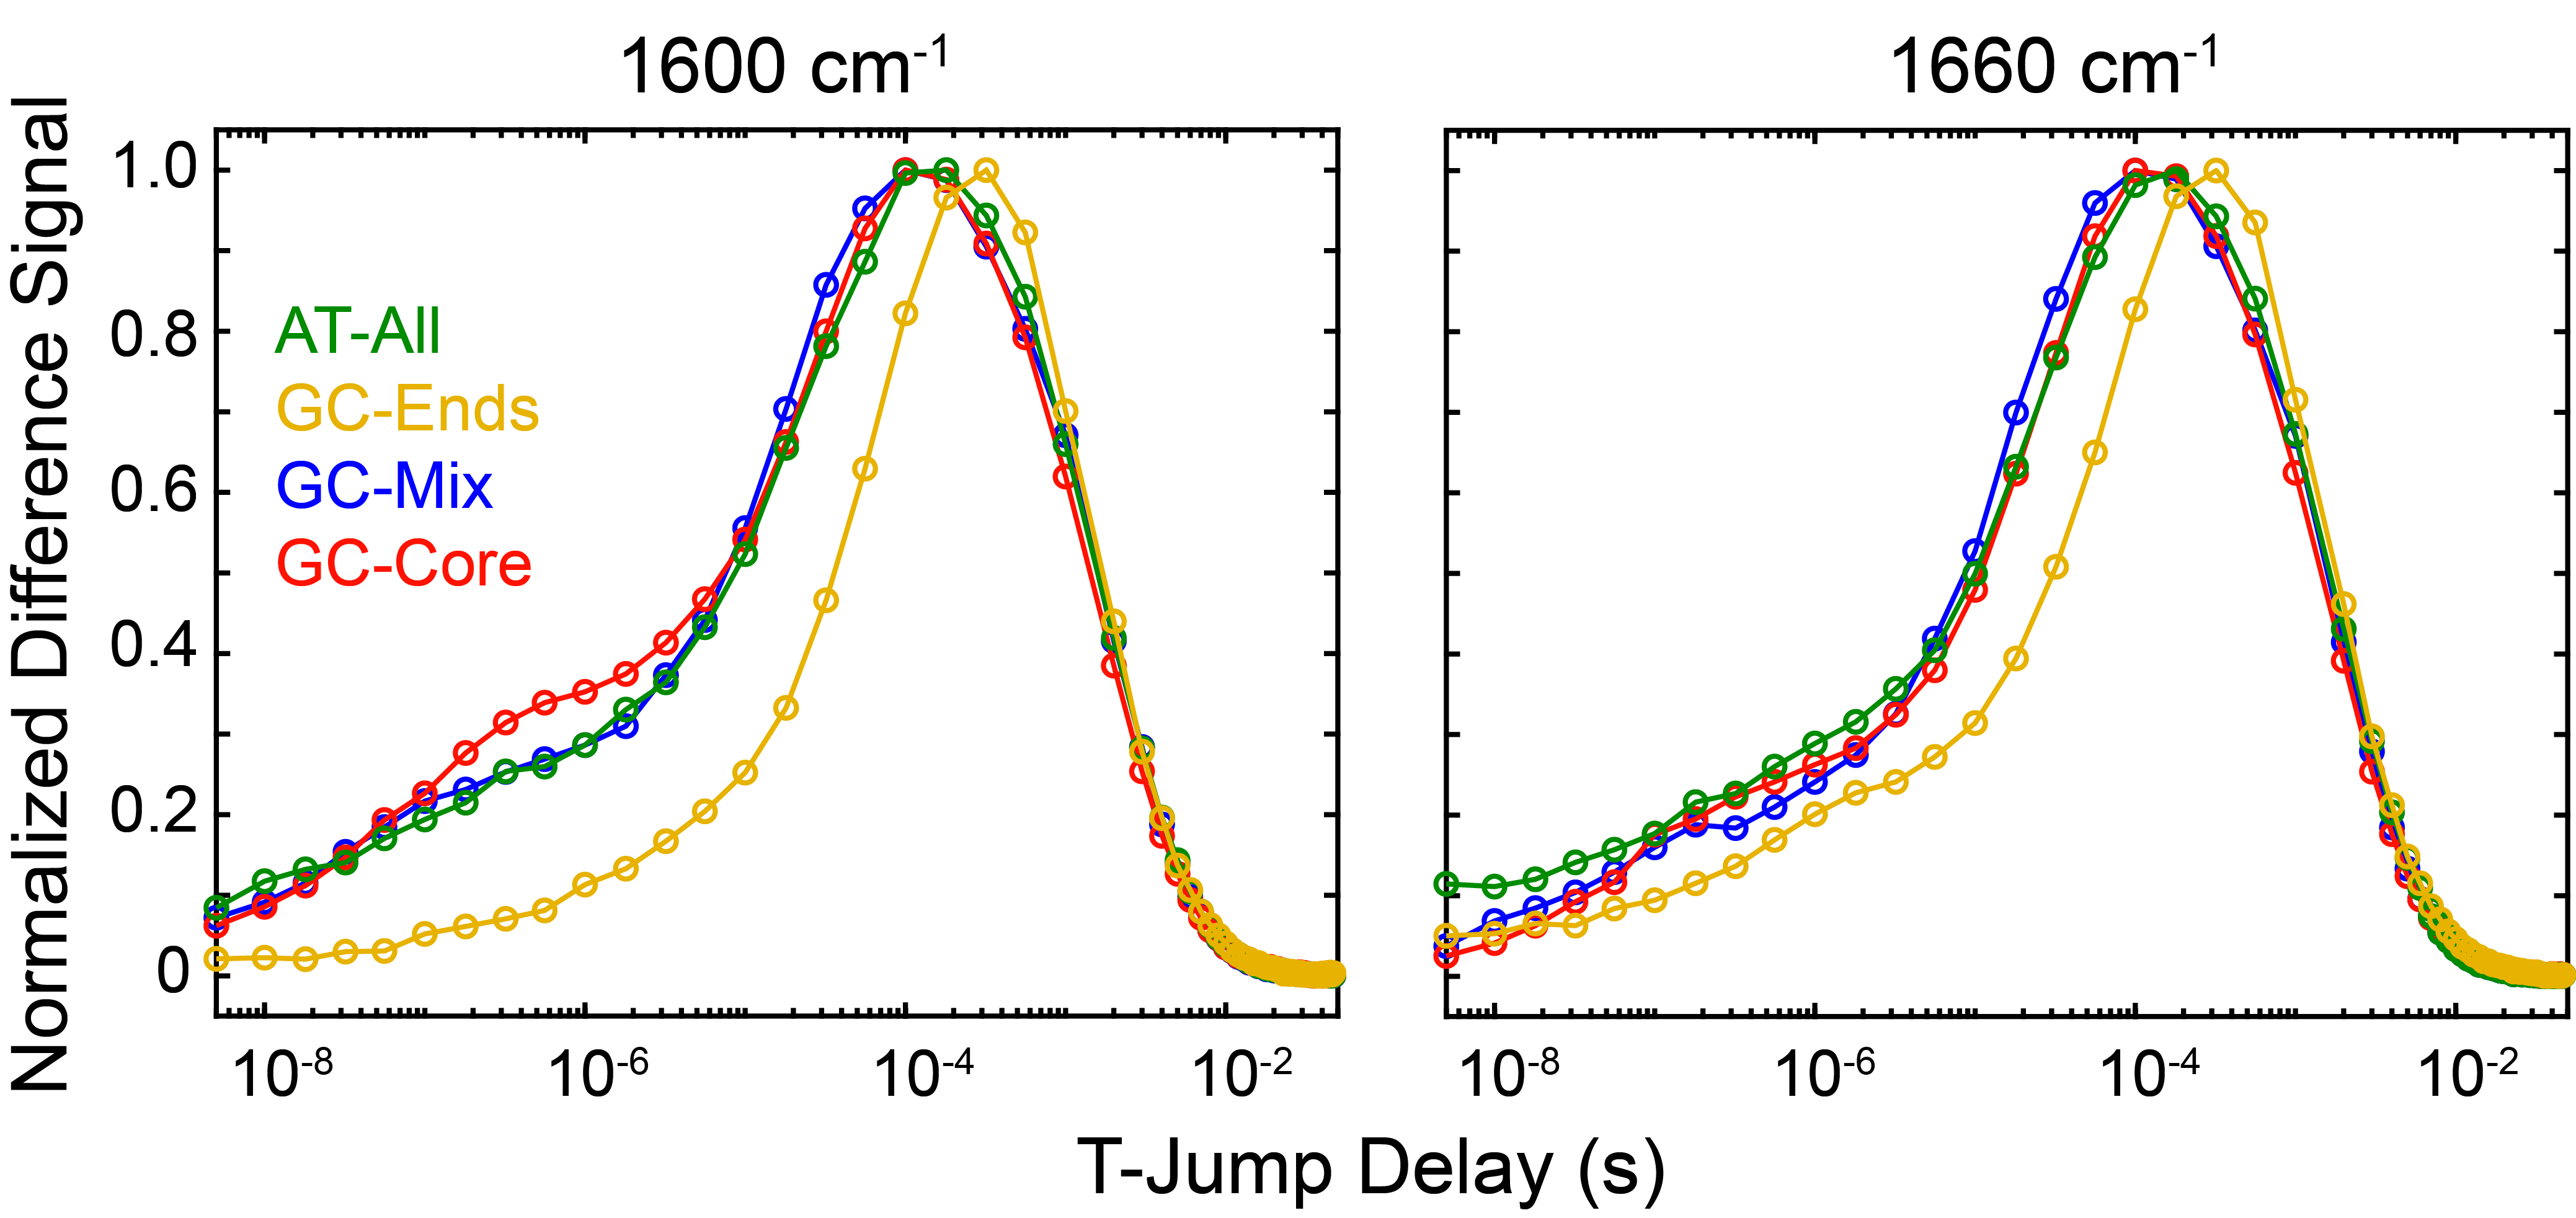
\includegraphics[width=120mm, 
        scale=0.5]{Figs/figs_imp/GCSeq_TJTraces.png}
        \caption{Kinetic traces of the fast spectroscopic response show varied degrees of shifting based on sequences. More info from Brennan on subtle differences here, discuss stretching coefficients? (could include this in main text as well)}
        \label{fig:fast_stretching}
	\end{center}
\end{figure}

\begin{figure}[ht!]
	\begin{center}
        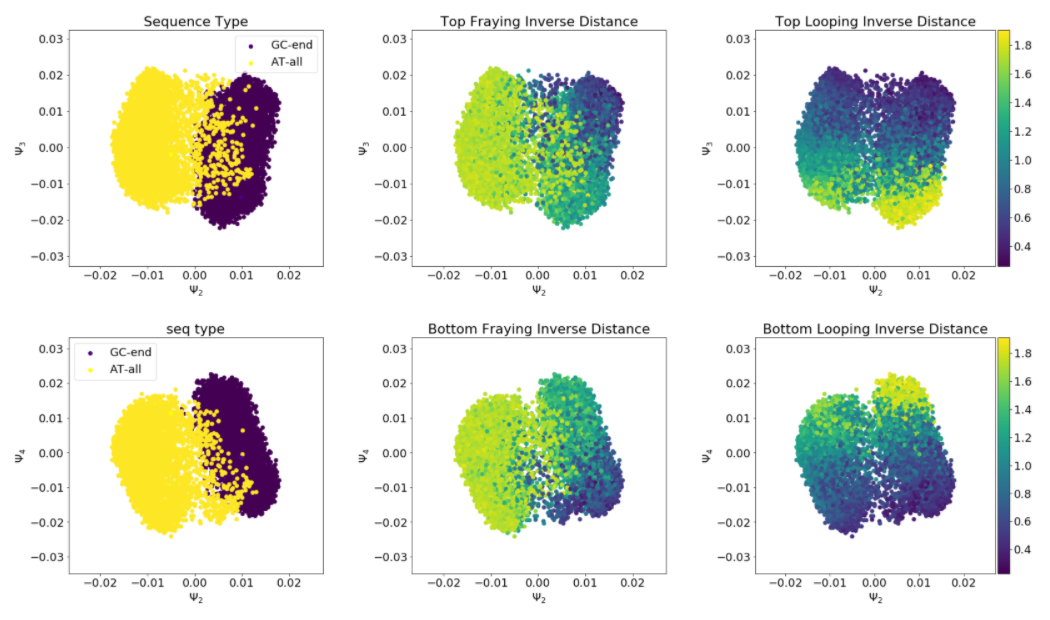
\includegraphics[width=\textwidth]{Figs/figs_imp/GC-end_dmaps_full.PNG}
        \caption{Full 5' diffusion maps including degenerate third diffusion map mode.}
        \label{fig:GC-end_dmaps_full}
	\end{center}
\end{figure}

\begin{figure}[ht!]
	\begin{center}
        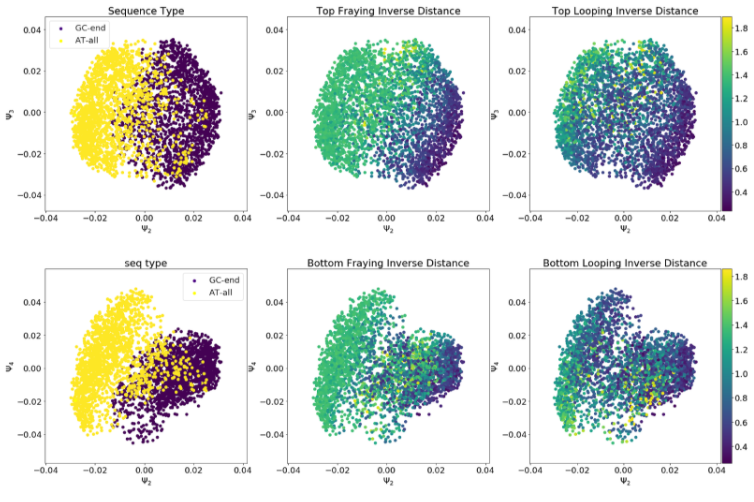
\includegraphics[width=\textwidth]{Figs/figs_imp/GC-end_dmaps_3prime.PNG}
        \caption{Full 3' diffusion maps, shows greater overlap between the AT-all and GC-end populations, as well as a less distinct "looping" region for intact GC bonds}
        \label{fig:GC-end_dmaps_3prime}
	\end{center}
\end{figure}

% add figure for slow and fast response fitting (just GC-core)
\begin{figure}[ht!]
	\begin{center}
        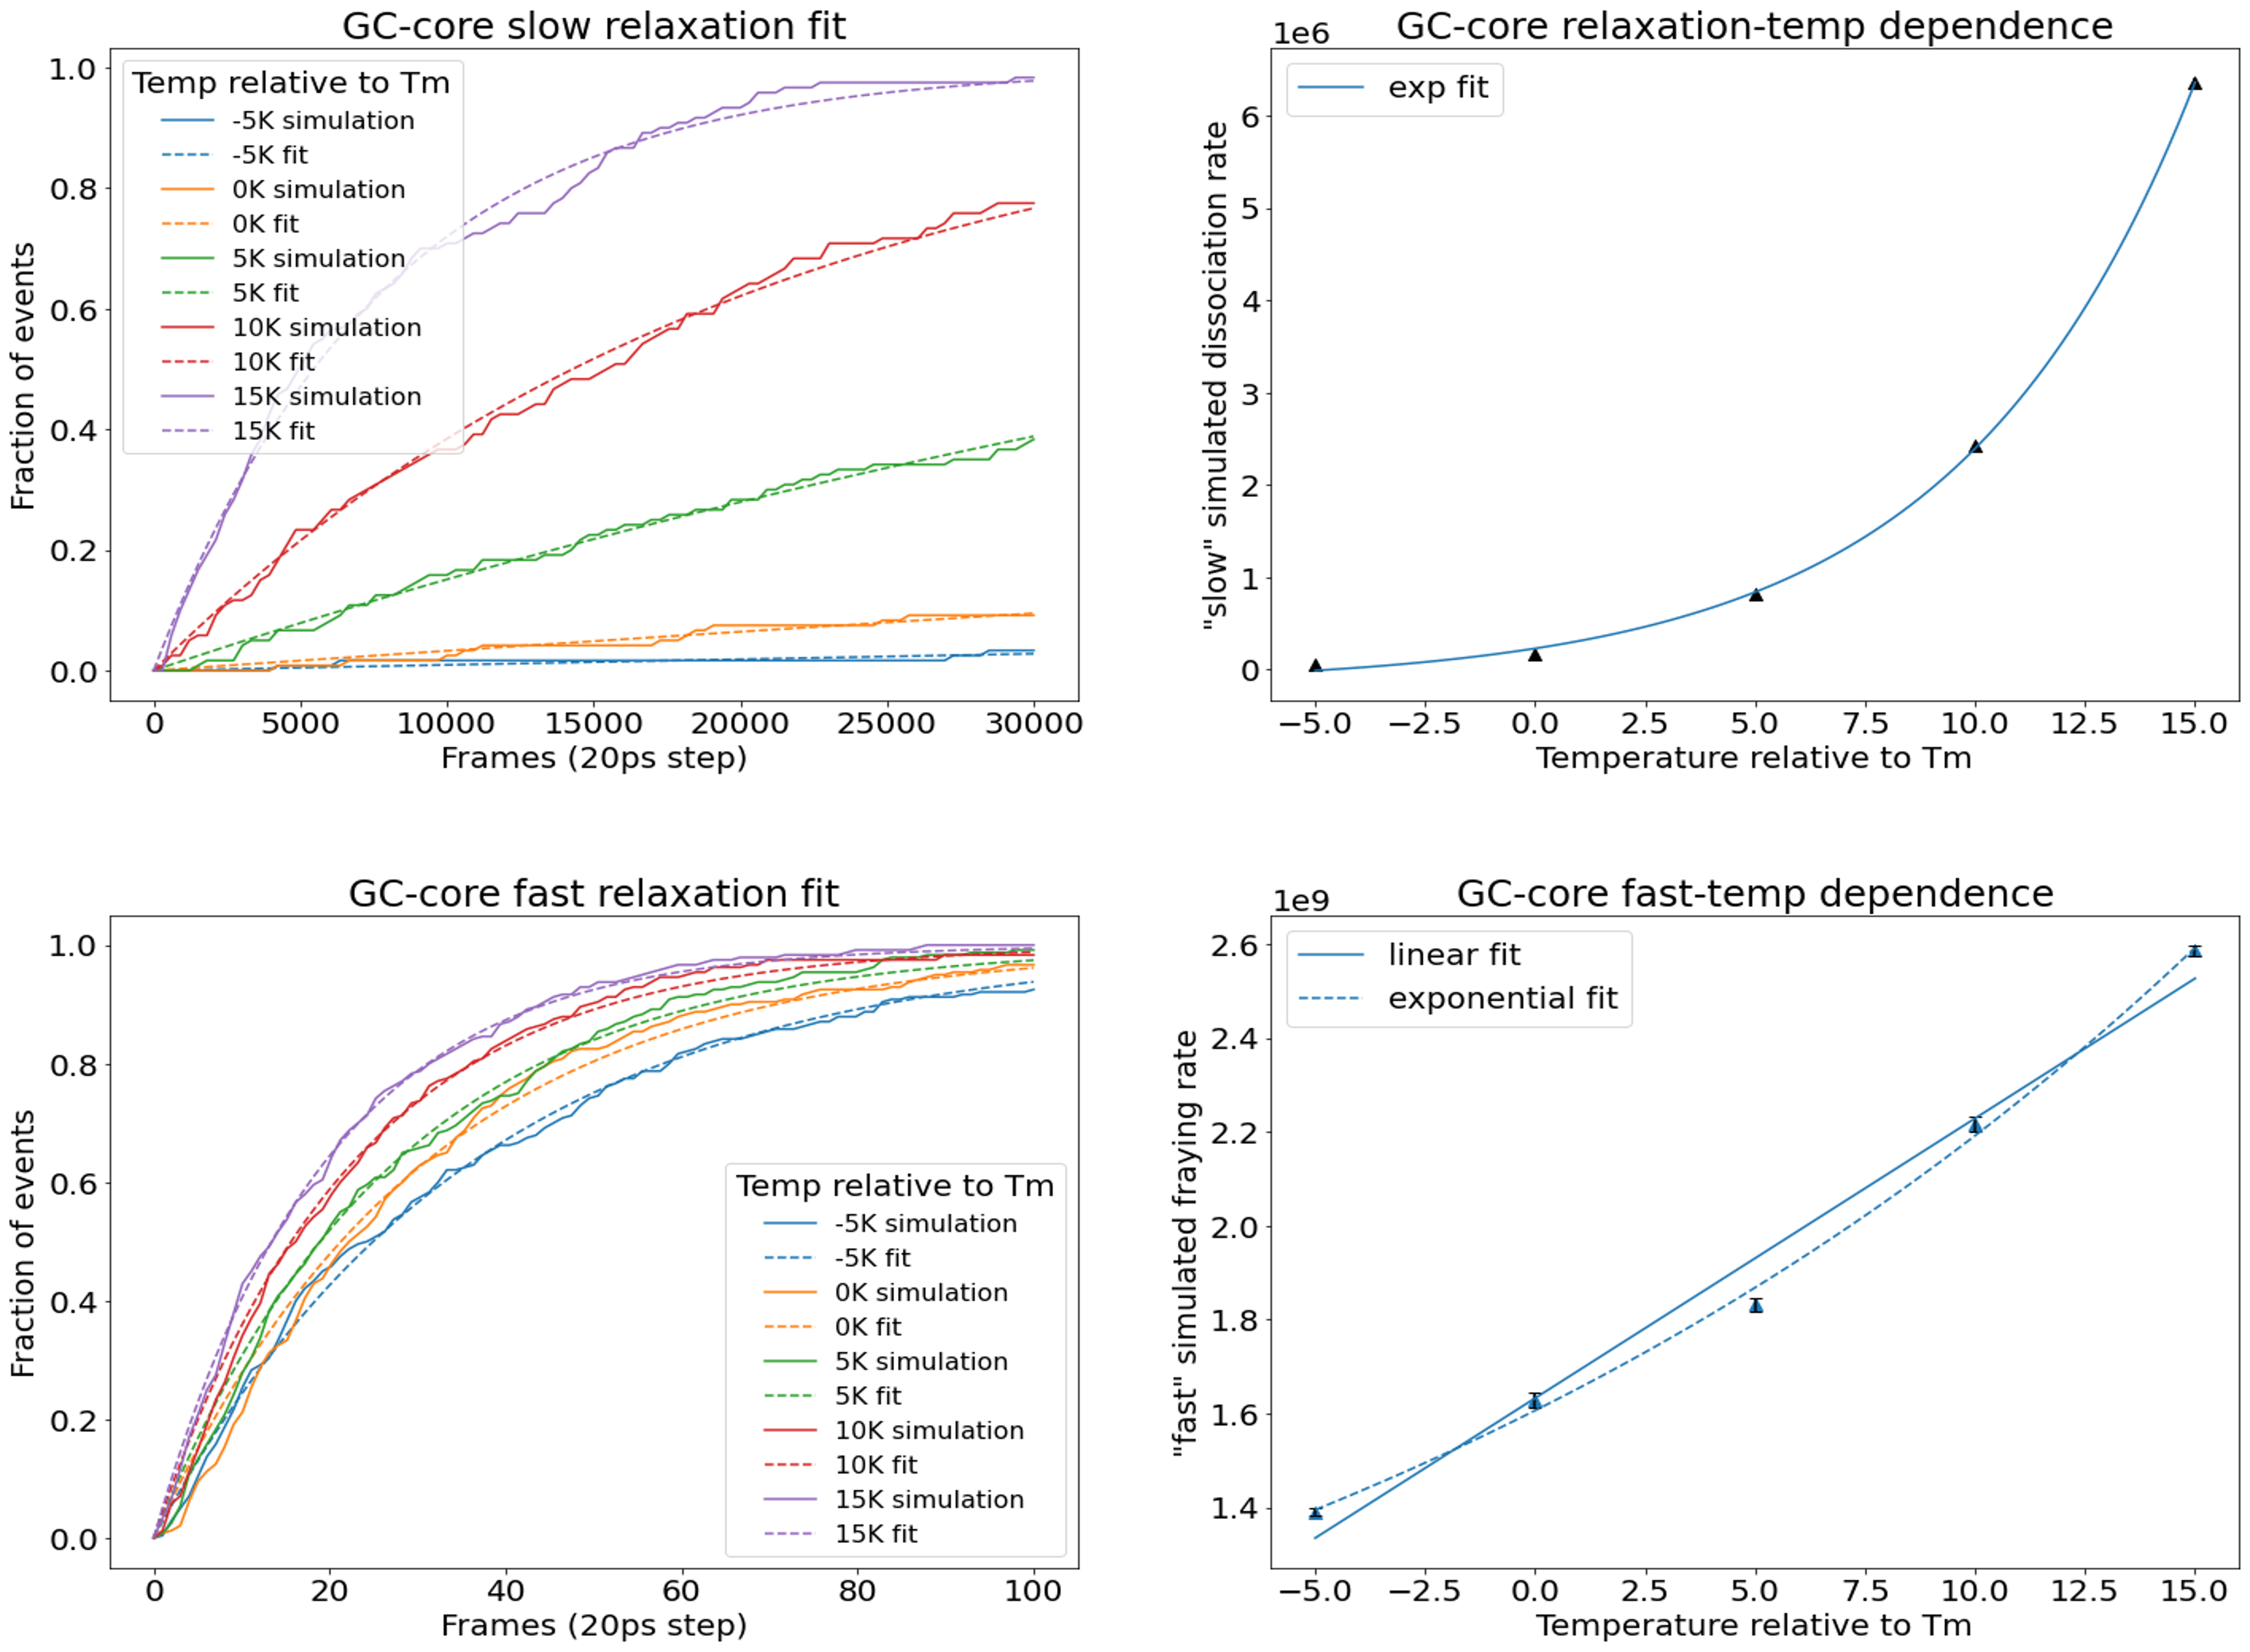
\includegraphics[width=\textwidth]{Figs/figs_imp/Tjump_fast_slow_fits.png}
        \caption{Slow and Fast modes were determined by fitting over a distribution of 120 independent simulations. For each temperature in the series, a relaxation curve was fit to the distribution and the associated exponential coefficient was used to the calculate rate. Temperatures series between -5 - +15K relative to empirically determined sequence melting temperature were explored. This process was repeated for each sequence (only GC-core is shown above).}
        \label{fig:fast_slow_fits}
	\end{center}
\end{figure}


%add anymore figures for the time analysis: As shown bleow:
\begin{comment}

\begin{figure}[ht!]
	\begin{center}
        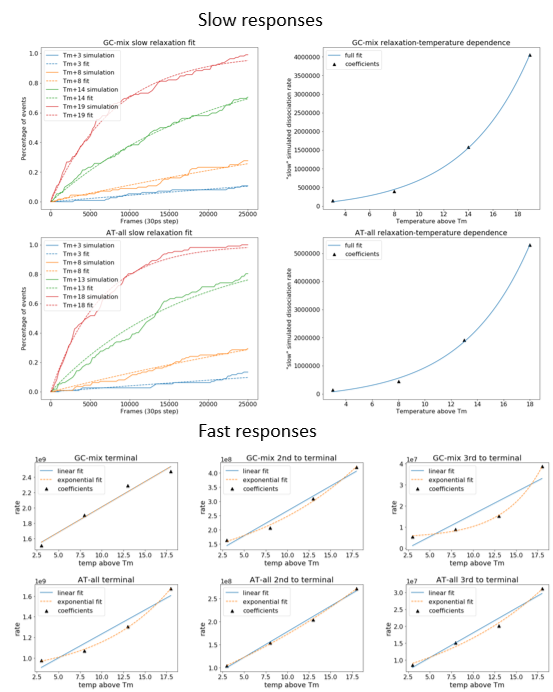
\includegraphics[width=\textwidth]{Figs/figs_0804/fast-slow_all-mix.png}
        \caption{Slow and Fast fits for GC-mix and AT-all, no acceleration values were calculated as there was not the same temperature-dependent data available for these sequences. GC-mix again shows barrierles fraying at the terminus, with a noticeable barrier for G:C bonds breaking at the second base pair in. AT-all shows a more exponential relationship for terminal fraying, likely because the simulations are run at lower relative temperatures.}
        \label{fig:relaxation-comparison_mix_and_all}
	\end{center}
\end{figure}

\begin{figure}[ht!]
	\begin{center}
        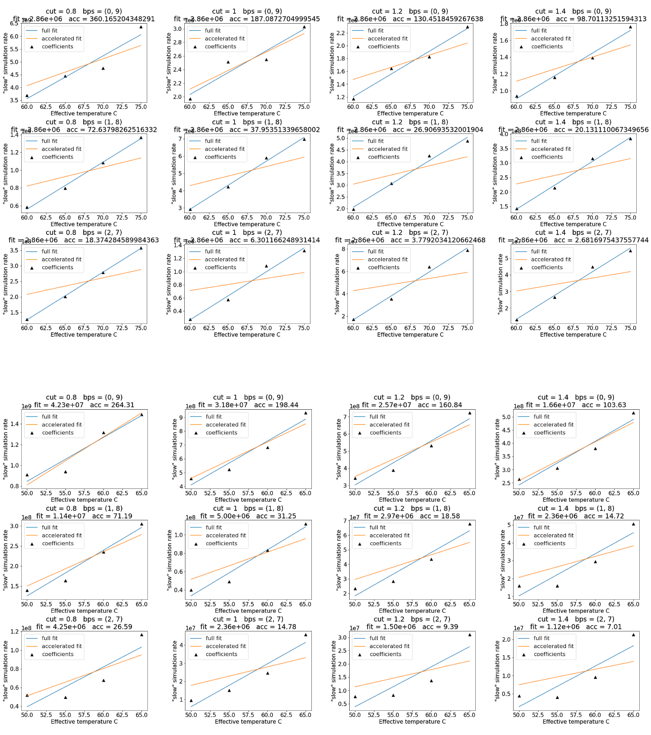
\includegraphics[width=\textwidth]{Figs/figs_0804/relaxation_core_and_end_allcuts.PNG}
        \caption{Fits across multiple cutoffs and basepairs for GC-core and GC-end fast response. (This is a placeholder until I reformat these to match the main text).}
        \label{fig:relaxation_core_and_end_allcuts}
	\end{center}
\end{figure}

\subsubsection{\label{sec:Results}Code to provide on GitHub} 
\begin{enumerate}
    \item Cross val data
    \item lammps run script and each sequence input files
    \item Featurization with mdtraj (reindexing and sparse saving)
    \item Dmaps for GC-core and GC-end
    \item timescales comparison
    \item SRV cross valss
    \item MSM construction
    
\end{enumerate}
\end{comment}

\begin{comment}

\section{\label{sec:Discussion}Discussion}

\citep{Galindo-Murillo2015ConvergenceDGCACGAACGAACGAACGC}
Long simulations shows that terminal fraying does not converge on the picosecond timescale

\citep{Nonin1995TerminalFraying}
Most simulations suppress fraying by placing GC pairs at termini.

\citep{Andreatta2006UltrafastHelix}
- Base opening process is slower than 40 ns but faster than 1ms
- Open termini state shows new fraying mode of 5ps (I think shows free base motions)
\end{comment}

\begin{comment}

%%%%%% Other MSM and timescales approaches  %%%%%%%%%%%

McGibbon, R. T., & Pande, V. S. (2015). Variational cross-validation of slow dynamical modes in molecular kinetics : Importance of not generating too many microstates and employting cross-validation to avoid artificially high scores or artificially slow dynamics. Both of these lead to models fitting statistical noise which is the root of boosted scores.

Pinamonti, G., Paul, F., Rodriguez, A., & Bussi, G. (n.d.). analyzed with core-set Markov state models, 43: Good ideas on core-based clustering. Assigning microstates based on physical characteristics is interesting but didn't seem to work for me in practice (could try doing this based on sim.log data with number of base pairs bound or some energy metric). Lot's of notes on this paper regarding comparisons to timescales. Good notes on higher resolution fraying interactions that we likely can't resolve.

Sua, E., Adelman, J. L., & Zuckerman, D. M. (2016). Accurate Estimation of Protein Folding and Unfolding Times : Beyond Markov State Models, 1. https://doi.org/10.1021/acs.jctc.6b00339:
More accurate ways to adapt MFPT into a rate

Refs for DNA fraying:
\citep{Hagan2003AtomisticDNA} Atomistic simulations for biosensign app (can include in intro). Use TPS to focus on kinetic pathway by which singl base pair bind/unbind. Focus on end base of 3-bp oligomer in explicit solvent. Finds order parameters tracking base pair binding as well as intra-strand stacking. (energy and distance for each). 

\citep{Wong2008TheSimulations} Three step melting process: untwisting most important,

6K.-Y. Wong and B. M. Pettitt, “The pathway of oligomeric DNA melting investigated by molecular dynamics simulations,” Biophys. J. 95, 5618– 5626 (2008).
37A. Perez and M. Orozco, “Real-time atomistic description of DNA unfold- ing,” Angew. Chem. 49, 4805–4808 (2010).
38M. F. Hagan, A. R. Dinner, D. Chandler, and A. K. Chakraborty, “Atomistic understanding of kinetic pathways for single base-pair binding and unbinding

\end{comment}


\clearpage
\newpage

%\bibliography{references}
\bibliography{refs_mendeley2}

%%%%%%%%%%%%%%%%%%%%%%%%%%%%%%%%%%%%%%%%%%%%%%%%%%%%%%%%%%%%%%%%%%%%%
%% The "tocentry" environment can be used to create an entry for the
%% graphical table of contents.
%%%%%%%%%%%%%%%%%%%%%%%%%%%%%%%%%%%%%%%%%%%%%%%%%%%%%%%%%%%%%%%%%%%%%

\clearpage


\end{document}
